\documentclass[review]{elsarticle}

\usepackage{lineno,hyperref}
\modulolinenumbers[5]


%%%%%%%%%%%%%%%%%%%%%%%
%% Elsevier bibliography styles
%%%%%%%%%%%%%%%%%%%%%%%
%% To change the style, put a % in front of the second line of the current style and
%% remove the % from the second line of the style you would like to use.
%%%%%%%%%%%%%%%%%%%%%%%

%% Numberedo
%\bibliographystyle{model1-num-names}\usepackage{amssymb}



\usepackage{amssymb}
%\usepackage{amsmath}
\usepackage{pslatex}
\usepackage[overlap,CJK]{ruby}
\usepackage{linguex}
%\usepackage[pdftex]{graphicx}
\usepackage{graphicx}
\usepackage{multirow}
\usepackage{subfigure}
\usepackage{paralist}

\newcommand{\hlc}[2][yellow]{ {\sethlcolor{#1} \hl{#2}} }
\usepackage{fixltx2e}

\usepackage{tabularx}

%% Numbered without titles
%\bibliographystyle{model1a-num-names}

%% Harvard
%\bibliographystyle{model2-names.bst}\biboptions{authoryear}

%% Vancouver numbered
%\usepackage{numcompress}\bibliographystyle{model3-num-names}

%% Vancouver name/year
%\usepackage{numcompress}\bibliographystyle{model4-names}\biboptions{authoryear}

%% APA style
%\bibliographystyle{model5-names}\biboptions{authoryear}

%% AMA style
%\usepackage{numcompress}\bibliographystyle{model6-num-names}

%% `Elsevier LaTeX' style
\bibliographystyle{elsarticle-num}
%%%%%%%%%%%%%%%%%%%%%%%%

\begin{document}

\begin{frontmatter}

\title{Combining Traditional Data Sources, Unmanned Aerial Vehicle Derived Data and Statistical Relational Learning to Improve Dengue Surveillance}

%\tnotetext[mytitlenote]{Fully documented templates are available in the elsarticle package on \href{http://www.ctan.org/tex-archive/macros/latex/contrib/elsarticle}{CTAN}.}

%% Group authors per affiliation:


\author[label1]{Raghvendra Jain}
\author[label2]{Sra  Sontisirikit}
\author[label3]{Sopon Iamsirithaworn}
\author[label4]{Marc Cavazza}
\author[label1]{Helmut Prendinger}

%\author[label3]{Klaus Br\"ugmann}

\address[label1]{{jain@nii.ac.jp, helmut@nii.ac.jp}\\
	National Institute of Informatics, \\
	2-1-2 Hitotsubashi, Chiyoda-ku, Tokyo, 101-8430, Japan\\}


\address[label2] {{arttioz@gmail.com} \\ 
	Asian Institute of Technology, School of Engineering and Technology, Thailand}

\address[label3]{{iamsiri@gmail.com}\\
	Department of Disease Control Thirteenth Division, Bangkok, Thailand}

\address[label4]{{M.O.Cavazza@kent.ac.uk} \\ 
	School of Engineering and Digital Arts, University of Kent} 





%\author{Raghvendra Jain \fnref{myfootnote}}  
%\address{Radarweg 29, Amsterdam}
%\fntext[myfootnote]{Since 1880.}
%
%%% or include affiliations in footnotes:
%\author[mymainaddress,mysecondaryaddress]{Elsevier Inc}
%\ead[url]{www.elsevier.com}
%
%\author[mysecondaryaddress]{Global Customer Service\corref{mycorrespondingauthor}}
%\cortext[mycorrespondingauthor]{Corresponding author}
%\ead{support@elsevier.com}
%
%\address[mymainaddress]{1600 John F Kennedy Boulevard, Philadelphia}
%\address[mysecondaryaddress]{360 Park Avenue South, New York}

\begin{abstract}
We present a machine learning-based methodology capable of providing real-time (“nowcast”) and forecast estimates of dengue prediction in the Thailand by leveraging data from multiple data sources including: survey data, hospital visit records and drone derived data.  Our main contribution consists of (a) addressing the limitations of the method for traditional data sources by combining it with the data derived using unmanned aerial vehicles (UAVs); and (b) understanding epidemiology using statistical relational learning techniques (SRLs). 

Our methodology enables...
We evaluate the predictive ability..
Our approach demonstrates several advantages: (1)...(2)..



%Our methodology exploits the information in each data source and produces accurate weekly predictions for up to four weeks ahead of the release of government reports. We evaluate the predictive ability of our ensemble approach during the 2013–2014 (retrospective) and 2014–2015 (live) flu seasons for each of the four weekly
%time horizons. 


%Our ensemble approach demonstrates several advantages: (1) our ensemble
%method’s predictions outperform every prediction using each data source independently,
%(2) our methodology can produce predictions one week ahead of GFT’s real-time
%estimates with comparable accuracy, and (3) our two and three week forecast estimates
%have comparable accuracy to real-time predictions using an autoregressive model. Moreover,
%our results show that considerable insight is gained from incorporating disparate data
%streams, in the form of social media and crowd sourced data, into influenza predictions in all
%time horizons.


\end{abstract}

\begin{keyword}
Dengue Foreccasting \sep Statistical Relational learning \sep Probabilistic Relational Modeling \sep Bayesian Epidemiology \sep Disease Surveillance \sep Unmanned Aerial Vehicles. 
\end{keyword}

\end{frontmatter}

\linenumbers

\section{Introduction}

Dengue, a mosquito borne viral disease, has been a significant cause of death and hospitalization among children in developing countries such as India, Thailand etc. Despite this, the surveillance for diagnosing dengue has been limited which makes it difficult to generate detailed information on its epidemiology.

%Therefore, the goal of this research is to create a system that can acquire detailed relevant information and use it to predict the occurrence of dengue within a geographical region, so that public health experts can prepare for, manage and control the epidemic.  
%
%There are two main problems to realize the goal: \\
%\textbf{Problem 1:} \textit{Limitations of the method for data acquisition}. To understand the epidemiology of dengue, data about the changes in relevant environmental factors such as land usage pattern, radiation, toxins, pollutants, humidity, temperature etc., is required. However, the data acquired via satellite has several limitations e.g. infrequent data acquisition, higher operating cost, low spatial resolution (highest resolution is 41 cms), cloud contamination, required expertise for data management etc. Thus, the spatial and temporal accuracy of such data is limited. \\
%\textbf{Problem 2:} \textit{Limitations of the method of understanding epidemiology characteristic}. The hypothesis-testing methods such as national surveys and randomized controlled trials do not incorporate (2.a) high-dimensional longitudinal observational data (2.b) frequent updates of the variations in data (2.c) inherent uncertainties of the data sources, or (2.d) probabilistic relationship between ‘expected’ causes and effects of spread of dengue virus. 
%
%\texttt{To realize the goal, our approach is \textbf{probabilistic relational modeling of dengue epidemiology using UAV-derived data}. It has two goals to solve two corresponding problems 1 and 2: \\
%\textbf{Goal 1:} Data acquisition using unmanned aerial vehicles (UAVs). The use of UAVs overcomes the limitations associated with satellite data. Using UAVs enables (a) mounting onboard various sensors for different purposes (b) acquiring data with high spatial resolution (typically of 4-20 cms) in real-time and at frequent time points (c) ease-of-use without a significant training or technical knowledge (d) capturing of ‘stereo’ images that can be used for 3D visualization of the landscape and feature extraction. \\
%\textbf{Goal 2:} Understanding epidemiology using probabilistic relational models (PRMs). Unlike a BN, the PRM allows a more compact representation of domain of environmental impact assessment, which involves various factors, their attributes and relationships among them.}



Dengue fever and dengue hemorrhagic fever (DF/DHF) result from infection by any of four serotypes of dengue viruses (DENV 1–4). The infection by one type usually gives lifelong immunity to that type, but only short-term immunity to the others. Transmission occurs through the bite of infected Aedes mosquitoes, principally Aedes aegypti. This kind of mosquito prefers to breed in areas of stagnant water, such as flower vases, uncovered barrels, buckets, and discarded tires, but the most dangerous areas are wet shower floors and toilet tanks, as they allow the mosquitoes to breed inside the residence. The number of cases of dengue fever has increased dramatically since the 1960s, with between 50 and 528 million people infected yearly. Hundreds of thousands of cases of dengue are reported each year in tropical regions of the Americas, Africa, Asia, and Oceania. Globally, more than 2.5 billion people are at risk \cite{whodengue2012}. The World Health Organization (WHO) estimates that more than 50 million dengue virus (DENV) infections and 20,000 dengue disease-related deaths occur annually worldwide \cite{world2007scientific,whodengue2012fact}, and a recent disease distribution model estimated that were 390 million DENV infections in 2010, including 96 million apparent infections. Overall, 70\% of these apparent infections occurred in Asia \cite{bhatt2013global}. In 2015, there were 111,826 reported cases in Thailand \cite{denguethai2015}. 
	
There have been numerous urban outbreaks of dengue with significant health and economic impact \cite{gubler2002epidemic,gubler2004cities,anuradha19981996,vaughn2000invited}. Studies in Thailand and Brazil have shown that the social and economic impact is equivalent to that of malaria in these countries \cite{clark2005economic,luz2009disability}. Dengue also poses a risk to those who travel to endemic areas and is increasingly being reported in travelers returning from trips to endemic countries \cite{farrar2007editorial}. However, globally, dengue research has not received the same level of funding as other tropical infectious diseases. There are currently no available drugs and no licensed vaccine. The main mosquito control methodology: reducing the habitat and the number of mosquitoes and limiting exposure to bites is currently the best method for disease prevention. 
	
This research will focus on analyzing captured data from UAVs sensors such as image to classified land-type, landmark, and weather for estimating infection factors from Aedes mosquito combined with population statistics in the target area to predict risk of dengue outbreak.
	\begin{figure}[htbp]
		\begin{center}
			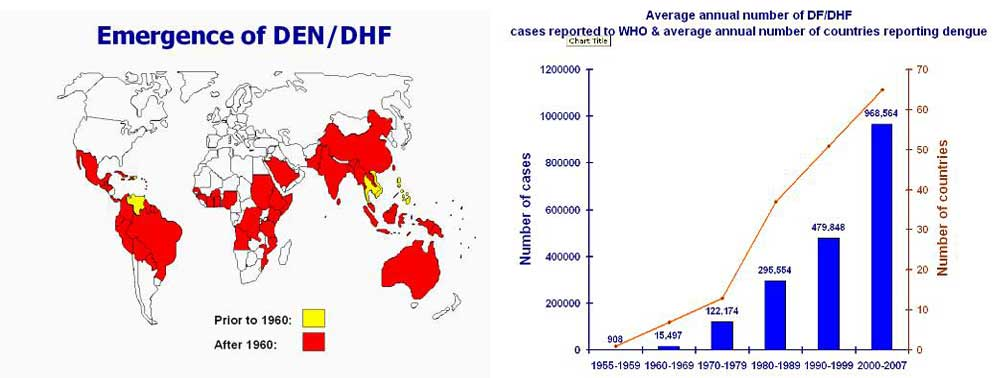
\includegraphics[width=150mm]{./figures/denguespread}
			\caption[Increase of dengue incidence rate from 1970-2007 in worldwide. Reprinted from the website of \protect\cite{whoimpactdengue2008}.]{The figure show the increase of incidence rate of dengue from 1970-2007. Before 1970, there are only 9 countries that experienced DHF cases. But in twenty-first century, the incident rate is increase dramatically and the disease is now endemic in more than 100 countries. Up to 50 million infections occur annually with 500 000 cases of DHF and 22,000 deaths mainly among children. The virus became the most important mosquito-borne viral disease in the world. Reprinted from the website of \protect\cite{whoimpactdengue2008}.}	
			\label{figure-denguespread}
		\end{center}
	\end{figure}
	%----------------------------------------------------------------------------------------------------------------------------------------------------------------------------------------
%\section{Problem Statement}

The risk of epidemic dengue transmission is determined by a combination of factors that include level of human immunity to virus serotypes, virulence characteristics of the virus strain, abundance of Aedes mosquitoes, weather, and population statistics in target area \cite{focks1995simulation}. Several potential predictive indicators for outbreaks have been described but further study is needed \cite{leitmeyer1999dengue,runge2008does,thammapalo2008environmental,sarfraz2014near}. Difference researches have identified different factors; those models need to be compared on common data sets. Furthermore, the appearance of a new dengue serotype can be used as an early warning sign for a possible outbreak but the association between the introduction of a new serotype and outbreak occurrence remain unknown \cite{de2004dengue}. The complexity and interdependence of the factors make prediction of the risk of a dengue outbreak very hard to estimate over short time scales. 
	
The main factors related to the abundance of Aedes mosquitoes in an area are related to the environment in the target area. The environment is continually changing depending on weather and human action. To gain  environment data, satellite imagery  is common and extremely useful tool for observing the area. However, a satellite imagery has long repeat times and low spatial resolution,we can never know with certainly the current environment of target area, and we lose detail. In order to gain fresh current data from a target area towards creating a high accuracy prediction, I will explore the use of UAVs to observe target areas to gain real time, high detail data for extraction of environment factors predictive of dengue outbreak.
	
%\section{Objectives}
	
%We study the environmental factors of dengue fever outbreak from dengue patients recoded data in Bangkok, Thailand. These data of each patient which can be used to study geographic factors related to dengue fever by mapping address locations to satellite imagery, then analyzing the common landmarks and land types that close to outbreak locations. The mosquito population is also highly dependent on climate.  In order to tackle this issues, we will need to divided the data in to set divided by district area. The analyzed data will be used to train and test for the prediction model. The second step of the project will be to identify  environmental factors that can be observed locally by a UAVs that are pertinent in the context of dengue. Some of the indices that we would like to study include: number of suspect areas that have Aedes mosquito lairs, humidity, air warmness, density of houses, quality of houses, level of precipitation, and so on. 
In this research we: 
	
	\begin{enumerate}
		\item Identify the environmental factors of dengue fever by environments of patient’s house and UAVs sensor data.
		
		\item Analyze the causes and consequences of existing dengue fever factors to calculate the possibility of dengue fever outbreaks in target area. 
		
		\item Build a new prototype system able to integrate data from multiple sensor platforms and data sources in order to measure the inputs to the model describes in objective above automatically. 
		
		\item Evaluate of the prototype combined with prediction model by surveying one village in Bangkok.
	\end{enumerate}
	
	%----------------------------------------------------------------------------------------------------------------------------------------------------------------------------------------



\section{Related Work}
%\label{ch:literature-review}
%
%
%\section{Environmental factors related to dengue outbreak}
%\label{section-enironmental-factor-of-dengue-outbreak}

There are several  environmental factors related to dengue outbreak that have been identified from case studies in Southeast Asia \cite{sulaiman1996relationship,thammapalo2008environmental,sarfraz2014near,nakhapakorn2005information}. There are many research  conclude that most dengue cases are occurred in urban areas due to various contributing factors such high population density, inadequate housing, and inappropriate human behavioral practices \cite{chang2009combining,knudsen1992vector,troyo2009urban}. 

% 2.3.1
\subsection{Vector surveillance}

Surveillance of Aedes mosquito density is important for construction models of dengue transmission, in order to prioritize areas and seasons for vector control. Selection of appropriate surveillance strategies is based upon the desired outcome or objective, also taking into consideration time, available resources, and infestation levels. Additionally, continued vector surveillance (as frequently as every seven days) is required to sustain the control measures and detect any increase in vector density. The 80\% of larvae or pupa in house are from Aedes mosquito. The most used indicators for vector surveillance are:

\textbf{Larval surveys:} Estimating presence of larvae and/or pupae of Aedes mosquitoes by surveying water-holding containers.

\textbf{House index (HI):} Percentage of houses infested with larvae and/or pupae.

\begin{equation}
\label{eq:hi}
HI =  \frac{\textrm{Number of houses positive for mosquito larvae or pupa}}{\textrm{Total number of houses surveyed}}  \times 100 
\end{equation}

\textbf{Container index (CI):} Percentage of water-holding containers infested with larvae or pupae.

\begin{equation}
\label{eq:ci}
CI =  \frac{\textrm{Number of wet containers found positive for mosquito larvae or pupa}}{\textrm{Total number of wet containers surveyed}}  \times 100 
\end{equation}

\textbf{Breteau index (BI):} Number of positive containers per house inspected.

\begin{equation}
\label{eq:bi}
BI =  \frac{\textrm{Number of wet containers found positive for mosquito larvae or pupa}}{\textrm{Total number of houses surveyed}}  \times 100 
\end{equation}

\textbf{Adult Aedes mosquitoes surveys:} Estimating adult Aedes mosquito population density using ovitraps, sticky traps, human landing collections \cite{barnard2014measurement}, or similar traps. 

%Figure \ref{figure-hi_bi_dengue_cases} shows the relationship between HI, BI, and dengue fever and dengue haemorrhagic fever cases in Kuala Lumpur city, Malaysia \cite{sulaiman1996relationship}. The correlation coefficient (r) of the relationship between BI and DF/DHF cases in each month was significant in the City Center zone, with a correlation coefficient at the 5\% level (r: 0.60, p \textless 0.05). However, in Jalan Klang Lama, Ceras, Setapak, Kepong, and Damansara zones, the correlation coefficient was not significant. Similarly, the correlation coefficient of the relationship between the HI and DF/DHF cases in each month was significant at the 2.5\% level (r  =  0.61, p \textless 0.025) but it was not significant in Jalan Klang Lama, Ceras, Setapak, Kepong, or Damansara.


%\begin{figure}[htbp]
%	\begin{center}
%		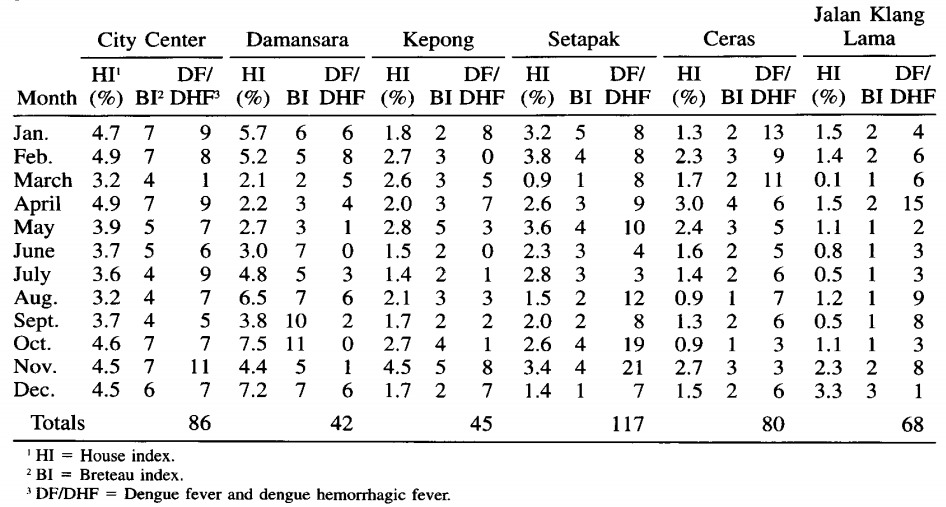
\includegraphics[width=140mm]{./figures/hi_bi_dengue_cases}
%		\caption{ Monthly Breteau and House indices of Aedes mosquito density and reported DF and DHF cases in six zones of Kuala Lumpur, Malaysia in 1994. Reprinted from \protect\cite{sulaiman1996relationship}.}
%		\label{figure-hi_bi_dengue_cases}
%	\end{center}
%\end{figure}

% 2.3.2
\subsection{Environmental factors and incidence of dengue fever and dengue haemorrhagic fever in urban Southern Thailand}

\cite{thammapalo2008environmental} analyze the spatial pattern of DF/DHF incidence at the district block level in Songkhla province, Thailand, to test the hypothesis that district block characteristics affect the incidence of the disease. There were 20,745 households with a population of 60,127 people. The main occupations of the population include trading, fishing, and government service. The municipality is divided into 146 districts, each containing about 140 houses and 400 residents. They aqquired data on the population, average number of people per house, children in each age group, and location data in Songkhla from the National Statistics Office, which had conducted a population census survey in 1997. Approximately 10\% of all the houses in each district were selected for the study of housing data which included: housing type, construction material, presence of water drainage, availability of window screens, waste disposal, and BI. 

The total number of houses visited was 1996. The overall percentages of infected people inhabiting shop-houses, single houses, buildings, slums and empty houses were 39\%, 37\%, 3\%, 5.4\% and 15.6\% respectively. The proportions of houses in which included people lived made of bricks, a mixture of brick and wood, wood, corrugated iron and others materials were 42\%, 28\%, 24\%, 3\%, and 2\%, respectively.

The results of the analysis housing factors vs. district incidence of DF/DHF: DF/DHF incidence per block had a positive correlation with the percentages of \textit{shop-houses, empty houses, brick-made houses and houses with poor garbage disposal}. A comparison of poor garbage disposal rate with DF/DHF is as shown in figure \ref{figure-house_with_garbage}. DF/DHF had a negative correlation with \textit{the average number of people per house, percentages of single houses, slum dwellings, wood-made houses and the BI}. 


%\begin{figure}[htbp]
%	\begin{center}
%		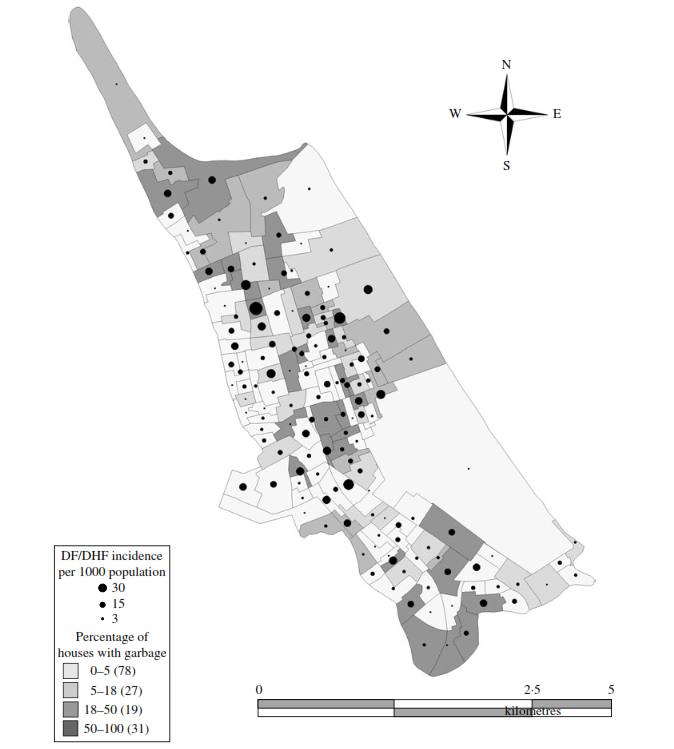
\includegraphics[width=110mm]{./figures/house_with_garbage}
%		\caption{DF/DHF incidence per 1000 population, compared to percentage of houses with poor garbage disposal in Songkhla municipality. Reprinted from \protect\cite{thammapalo2008environmental}.}
%		\label{figure-house_with_garbage}
%	\end{center}
%\end{figure}


% \begin{figure}[htbp]
% \begin{center}
% 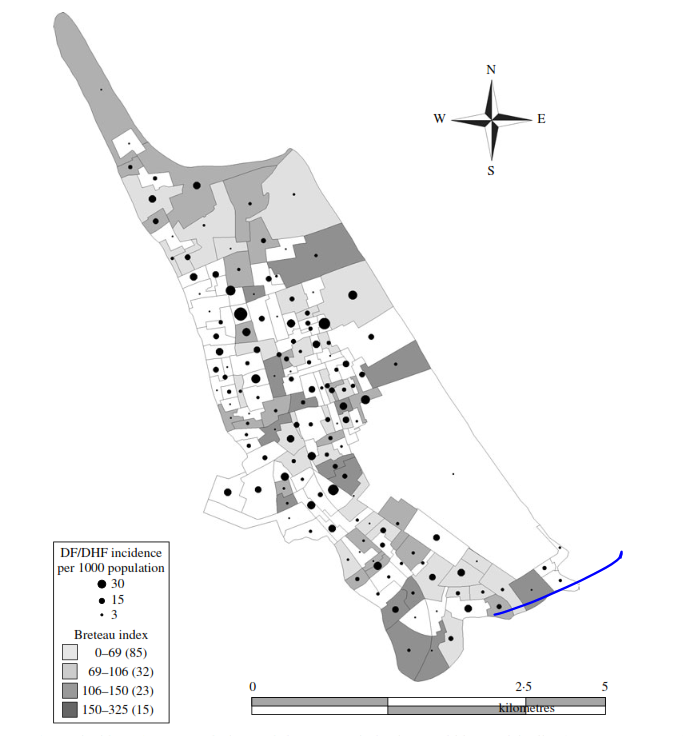
\includegraphics[width=110mm]{./figures/breteau_index}
% \caption{ DF/DHF incidence/1000 population rate and the Breteau index in Songkhla municipality. Reprinted from \protect\cite{thammapalo2008environmental}.}
% \label{figure-breteau_index}
% \end{center}
% \end{figure}

% 2.3.3
\subsection{Near real-time characterization of urban environments: a holistic approach for monitoring dengue fever risk areas: A city of Phitsanulok Province, Thailand}

\cite{sarfraz2014near} extract land-use types using object-based and spatial metric approaches to explore dengue incidence in relation to the surrounding environment in near real-time using Google and Advanced Land Observation Satellite images. Geospatial analysis on public health data indicated that most of the dengue cases were found in densely populated areas \textit{surrounded by dense vegetation}. Dense vegetation can facilitate the invasion of Aedes mosquitoes by providing abundant resting sites. 

Figure \ref{figure-gps_map_den_cases} shows the incidence of dengue cases in the city of Phitsanulok in 2010 in relation to important landmarks, for example, a hospital, market, temple and school. A positive relationship between dengue cases and neighborhoods was observed based on proximity and spatial analysis. \textit{Proximity analysis} indicated that most of the dengue cases were around \textit{institutions (40\%), religious places (18\%), and markets (15\%)}. The study also reports that dengue incidence was more prevalent in people of 5-24 years of age (67\%), while in terms of occupation, mostly \textit{students, the unemployed, laborers, and farmers (88\%)} were affected.


%\begin{figure}[htbp]
%	\begin{center}
%		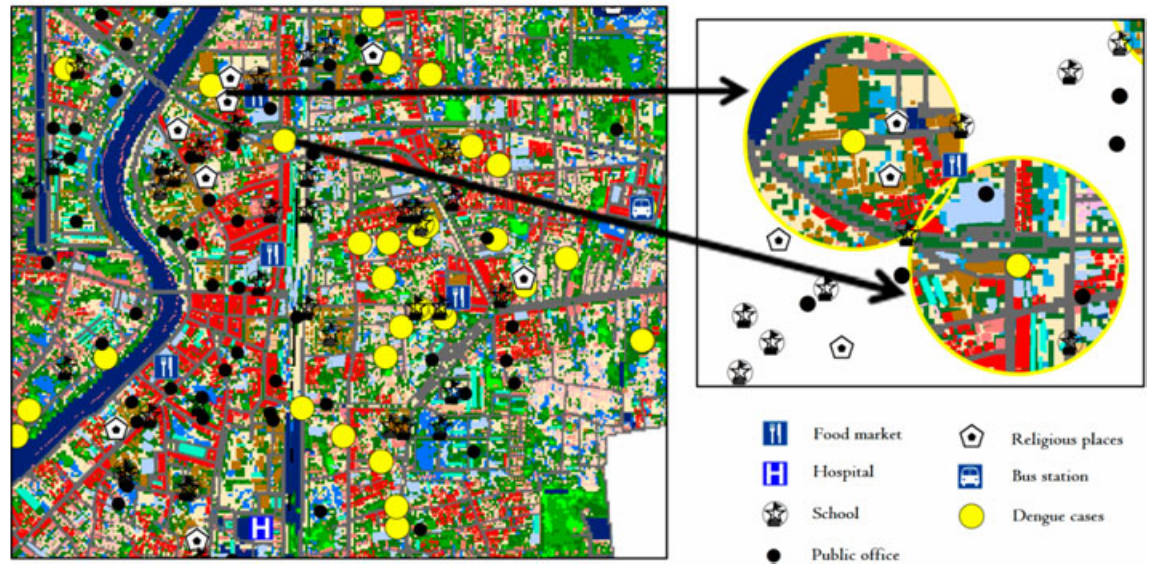
\includegraphics[width=110mm]{./figures/gps_map_den_cases}
%		\caption{ Location of dengue cases (yellow points) in Phitsanulok study area overlaid onto the land-use/land-
%			cover map. Reprinted from \protect\cite{sarfraz2014near}.}
%		\label{figure-gps_map_den_cases}
%	\end{center}
%\end{figure}

% 2.3.4
\subsection{An information value based analysis of physical and climatic factors affecting dengue fever and dengue haemorrhagic fever incidence: Sukhothai province, Thailand.}
\label{subsection-regressions-paper}

\cite{nakhapakorn2005information} explores empirical relationship of climatic factors rainfall, temperature and humidity with the DF/DHF incidences using multivariate regression analysis. Sukhothai province located in the northern Thailand, was selected as the study area for this work.  The province has a population of about 521,219. Climate of this area is subtropical with extreme high temperatures rising to 42$^{\circ}$C in April and dipping low up to 13.2$^{\circ}$C in December. Medical data were collected from the Provincial Health Office, Thailand, which collects monthly district level data.  

The purpose of the multiple regressions was to learn more about the relationship between several independent or predictor variables and the dependent or criterion variable (number of DF/DHF cases). 
In general, multiple regression procedures estimate a linear equation of the form:

\begin{equation}
\label{eq:linear}
Y\ =   (B\textsubscript{\textit{0}}) + (B\textsubscript{\textit{1}})(X\textsubscript{\textit{1}}) + (B\textsubscript{\textit{2}})(X\textsubscript{\textit{2}}) + ... + (B\textsubscript{\textit{k}})(X\textsubscript{\textit{k}}) 
\end{equation}

Where k is the number of predictors. Rainfall (R), temperature (T), and relative humidity (H) were considered as the independent variables. There are many related studies also conclude that climate is related to dengue outbreak \cite{li1985rainfall,hales2002potential,rueda1990temperature,tun2000effects,brady2013modelling}. The realtime at time T relationship (ER) between number of DF/DHF cases and the climatic data  (T\textsubscript{\textit{t}}, R\textsubscript{\textit{t}} and H\textsubscript{\textit{t}} ) at time \textit{t} during 5 years is listed in ER-1, ER-2, and ER-3 equations. Multiple regression analysis is employed to develop an empirical model to predict the dengue incidences by using the occurrence of DF/DHF cases and monthly climatic data of 5 years (1997$-$2001).

%\begin{figure}[htbp]
%	\begin{center}
%		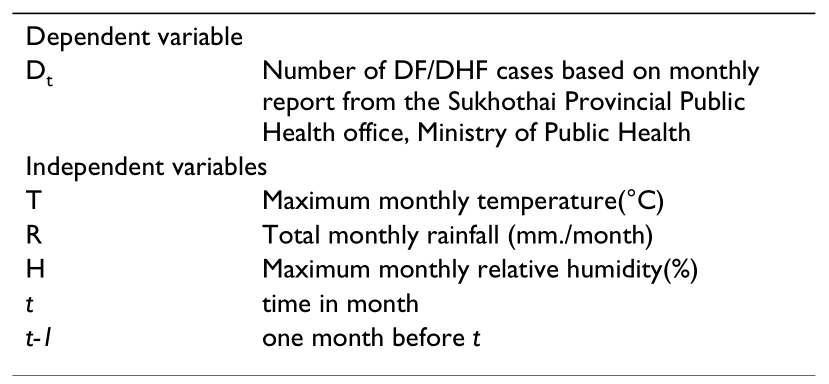
\includegraphics[width=110mm]{./figures/variable}
%		\caption{ Variables in the Sukhothai DF/DHF multiple regression study. Reprinted from \protect\cite{nakhapakorn2005information}.}
%		\label{figure-variable}
%	\end{center}
%\end{figure}
%
%\textbf{ER-1 equation:} 
%\begin{equation}
%\label{eq:er-1}
%D\textsubscript{\textit{t}} =   1408.318 + 0.151(R\textsubscript{\textit{t}}) - 4.368(T\textsubscript{\textit{t}})-12.798(H\textsubscript{\textit{t}} )
%\end{equation}
%
%The coefficient of determination ($R^2$) of ER-1 was 0.43.
%Multiple regression analysis was carried out for the occurrence of DF/DHF cases for the rainy season.
%
%\textbf{ER-2 equation:} 
%\begin{equation}
%\label{eq:er-2}
%D\textsubscript{\textit{t}} =   -13.893 + 0.377(R\textsubscript{\textit{t}}) + 1.3444(T\textsubscript{\textit{t}}) - 0.276(H\textsubscript{\textit{t}} )
%\end{equation}
%The coefficient of determination ($R^2$) of ER-2 was 0.62.
%
%According to the development period from a mosquito egg to the human disease, there is a time lag of about one month that leads to DF/DHF cases occurring in 7 - 45 days. The duration of larvae stages is 7 to 12 days, and the lifespan of the female mosquito is about 8 to 15 days. In the meantime, the virus develops in the mosquito for a period of 8$–$10 days. By the time a person infected with dengue virus develops fever, the infection is usually widely disseminated to many people. The virus is found in serum or plasma, in circulating blood cells and in selected tissues, especially those of the immune system, for approximately 2–7 days, roughly corresponding to the period of fever. Thus, DF/DHF cases at time t (in month e.g. May) depend on others factors at time t-1 (i.e. one month before month).
%
%The Empirical Relationship-3 (ER-3) with a one-month time lag as shown below offered a coefficient of determination ($R^2$) as 0.81. Therefore, the ER-3 was selected to model the DF/DHF incidence in Sukhothai as the closest output to the actual data during rainy season and the results were validated with 1998 data, as shown in Figure \ref{figure-er_3}.
%
%\textbf{ER-3 equation:} 
%\begin{equation}
%\label{eq:er-3}
%D\textsubscript{\textit{t}} =   621.824 + 0.345(R\textsubscript{\textit{t-1}}) - 0.609(T\textsubscript{\textit{t-1}}) - 6.321(H\textsubscript{\textit{t-1}} )
%\end{equation}
%
%\begin{figure}[htbp]
%	\begin{center}
%		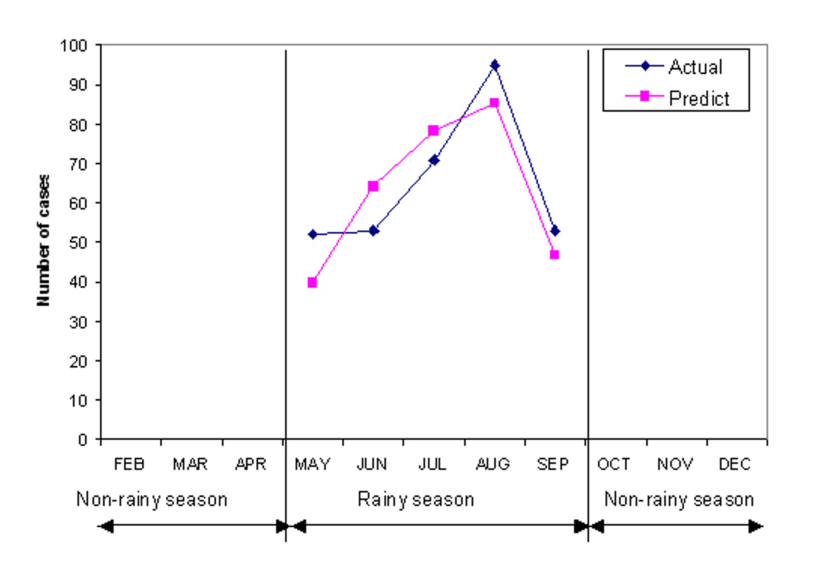
\includegraphics[width=110mm]{./figures/er_3}
%		\caption{ The relationship between actual and forecasted DF/DHF cases in Sukhothai, Thailand in 1998 during rainy season using ER-3. Reprinted from \protect\cite{nakhapakorn2005information}.}
%		\label{figure-er_3}
%	\end{center}
%\end{figure}

% 2.3.5
\subsection{Impact of daily temperature fluctuations on dengue virus transmission by Aedes aegypti.}

The diurnal temperature range (DTR) is the difference between the daily maximum and minimum temperature. \cite{lambrechts2011impact} show that DTR affects two important parameters underlying dengue virus (DENV) transmission by Aedes mosquito.

They evaluated experimentally the effect of DTR on the potential for DENV transmission by Aedes mosquito females under three temperature. Each experiment had the same average temperature (26 °C), but a different amplitude of daily temperature variation; control (DTR = 0$^{\circ}$C), moderate (DTR = 10$^{\circ}$C), and large (DTR = 20$^{\circ}$C). In two independent experiments using different DENV serotypes (DENV-1 and DENV-2), mosquitoes were less susceptible to virus infection and died faster under larger DTR (20$^{\circ}$C).  A thermodynamic model predicted that at mean temperatures <18 $^{\circ}$C, DENV transmission increases as DTR increases, whereas at mean temperatures >18 $^{\circ}$C, larger DTR reduces DENV transmission.

Infection analysis is divided in to two experiments. In the first experiment, rates of infection by a DENV-2 isolate were measured in a total of 525 Aedes mosquito females (175 in each of the three temperature regimes). Result of the first experiment is 97.1\%, 94.9\%, and 78.9\% of females were DENV-2 infected under DTRs of 0 °C, 10 °C, and 20 °C, respectively. In the second experiment, rates of infection by a DENV-1 isolate were measured in 227 Aedes mosquito females (132 in each of the two temperature regimes: low and large DTR regime) Result of the second experiment is, 97.0\% and 88.4\% of females were DENV-1 infected under DTRs of 0 °C and 20 °C, respectively.

Survival analysis is also divided in to two experiments. A total of 900 Aedes mosquito females were included in survival analysis in the first experiment with DENV-2, which 244 died during the course of the experiment. Mean survival times were 27.6, 27.9, and 27.3 days post infection under DTRs of 0 °C, 10 °C, and 20 °C, respectively. Although mean survival times were similar across DTR regimes, only ∼30\% of females under the DTR of 20$^{\circ}$C survived to the end of the experiment, compared with 50\% and ∼70\% under a DTR of 10$^{\circ}$C and 0$^{\circ}$C, respectively. 

%Survival results of the first experiment were confirmed in the second experiment with DENV-1. A total of 317 Aedes mosquito females were included in survival analysis, which 85 died during the course of the experiment. Mean survival times were 28.5 and 22.2 dpi under DTRs of 0 °C and 20 °C, respectively. This experiment conclude that DTR had a statistically significant influence on survival rates as shown in Figure \ref{figure-survive}.
%
%\begin{figure}[htbp]
%	\begin{center}
%		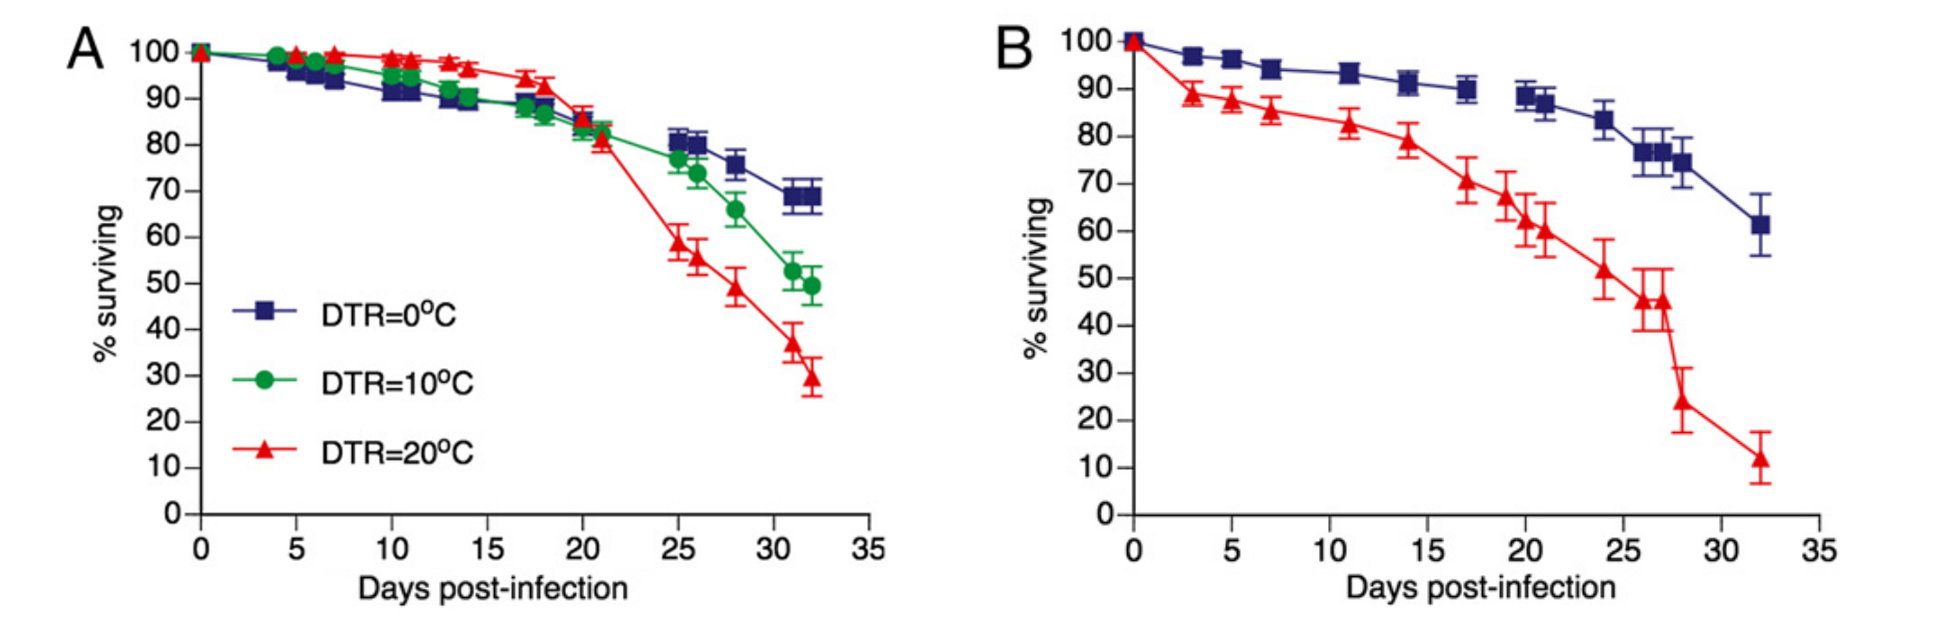
\includegraphics[width=150mm]{./figures/survive}
%		\caption[Effect of DTR on experimental survival of Aedes mosquito females after infected to DENV, Reprinted from \protect\cite{lambrechts2011impact}.]{ Effect of DTR on experimental survival of Aedes mosquito females after infected to DENV. 
%			In A, mosquitoes were exposed to a DENV-2 isolate. Survival curves are significantly different according to log-rank tests (overall: P < 0.0001; DTR = 0$^{\circ}$C vs. DTR = 10$^{\circ}$C: P = 0.0249; DTR = 10$^{\circ}$C vs. DTR = 20$^{\circ}$C: P = 0.0068). In B, mosquitoes were exposed to a DENV-1 isolate. Survival curves are significantly different according to a log-rank test (P < 0.0001). Reprinted from \protect\cite{lambrechts2011impact}.}
%		\label{figure-survive}
%	\end{center}
%\end{figure}
%\section{Environmental factors related to dengue outbreak}
%\label{section-enironmental-factor-of-dengue-outbreak}
%
%In this section will describes environmental factors related to dengue outbreak that have been identified from case studies in Southeast Asia \cite{sulaiman1996relationship,thammapalo2008environmental,sarfraz2014near,nakhapakorn2005information}. There are many research  conclude that most dengue cases are occurred in urban areas due to various contributing factors such high population density, inadequate housing, and inappropriate human behavioral practices \cite{chang2009combining,knudsen1992vector,troyo2009urban}. 

% 2.3.1
\subsection{Vector surveillance}

Surveillance of Aedes mosquito density is important for construction models of dengue transmission, in order to prioritize areas and seasons for vector control. Selection of appropriate surveillance strategies is based upon the desired outcome or objective, also taking into consideration time, available resources, and infestation levels. Additionally, continued vector surveillance (as frequently as every seven days) is required to sustain the control measures and detect any increase in vector density. The 80\% of larvae or pupa in house are from Aedes mosquito. The most used indicators for vector surveillance are:

\textbf{Larval surveys:} Estimating presence of larvae and/or pupae of Aedes mosquitoes by surveying water-holding containers.

\textbf{House index (HI):} Percentage of houses infested with larvae and/or pupae.

\begin{equation}
\label{eq:hi}
HI =  \frac{\textrm{Number of houses positive for mosquito larvae or pupa}}{\textrm{Total number of houses surveyed}}  \times 100 
\end{equation}

\textbf{Container index (CI):} Percentage of water-holding containers infested with larvae or pupae.

\begin{equation}
\label{eq:ci}
CI =  \frac{\textrm{Number of wet containers found positive for mosquito larvae or pupa}}{\textrm{Total number of wet containers surveyed}}  \times 100 
\end{equation}

\textbf{Breteau index (BI):} Number of positive containers per house inspected.

\begin{equation}
\label{eq:bi}
BI =  \frac{\textrm{Number of wet containers found positive for mosquito larvae or pupa}}{\textrm{Total number of houses surveyed}}  \times 100 
\end{equation}

\textbf{Adult Aedes mosquitoes surveys:} Estimating adult Aedes mosquito population density using ovitraps, sticky traps, human landing collections \cite{barnard2014measurement}, or similar traps. 

%Figure \ref{figure-hi_bi_dengue_cases} shows the relationship between HI, BI, and dengue fever and dengue haemorrhagic fever cases in Kuala Lumpur city, Malaysia \cite{sulaiman1996relationship}. The correlation coefficient (r) of the relationship between BI and DF/DHF cases in each month was significant in the City Center zone, with a correlation coefficient at the 5\% level (r: 0.60, p \textless 0.05). However, in Jalan Klang Lama, Ceras, Setapak, Kepong, and Damansara zones, the correlation coefficient was not significant. Similarly, the correlation coefficient of the relationship between the HI and DF/DHF cases in each month was significant at the 2.5\% level (r  =  0.61, p \textless 0.025) but it was not significant in Jalan Klang Lama, Ceras, Setapak, Kepong, or Damansara.
%
%
%\begin{figure}[htbp]
%	\begin{center}
%		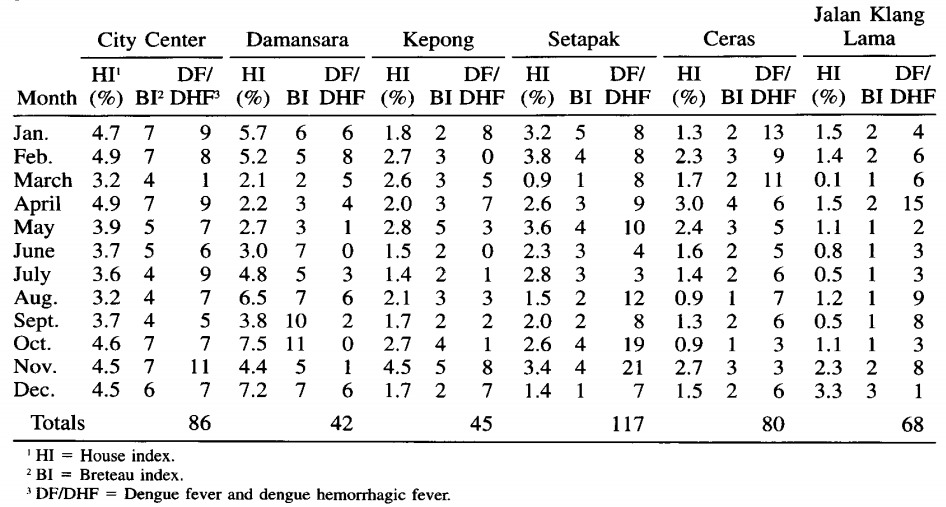
\includegraphics[width=140mm]{./figures/hi_bi_dengue_cases}
%		\caption{ Monthly Breteau and House indices of Aedes mosquito density and reported DF and DHF cases in six zones of Kuala Lumpur, Malaysia in 1994. Reprinted from \protect\cite{sulaiman1996relationship}.}
%		\label{figure-hi_bi_dengue_cases}
%	\end{center}
%\end{figure}

% 2.3.2
\subsection{Environmental factors and incidence of dengue fever and dengue haemorrhagic fever in urban Southern Thailand}

\cite{thammapalo2008environmental} analyze the spatial pattern of DF/DHF incidence at the district block level in Songkhla province, Thailand, to test the hypothesis that district block characteristics affect the incidence of the disease. There were 20,745 households with a population of 60,127 people. The main occupations of the population include trading, fishing, and government service. The municipality is divided into 146 districts, each containing about 140 houses and 400 residents. They aqquired data on the population, average number of people per house, children in each age group, and location data in Songkhla from the National Statistics Office, which had conducted a population census survey in 1997. Approximately 10\% of all the houses in each district were selected for the study of housing data which included: housing type, construction material, presence of water drainage, availability of window screens, waste disposal, and BI. 

The total number of houses visited was 1996. The overall percentages of infected people inhabiting shop-houses, single houses, buildings, slums and empty houses were 39\%, 37\%, 3\%, 5.4\% and 15.6\% respectively. The proportions of houses in which included people lived made of bricks, a mixture of brick and wood, wood, corrugated iron and others materials were 42\%, 28\%, 24\%, 3\%, and 2\%, respectively.

The results of the analysis housing factors vs. district incidence of DF/DHF: DF/DHF incidence per block had a positive correlation with the percentages of \textit{shop-houses, empty houses, brick-made houses and houses with poor garbage disposal}.
% A comparison of poor garbage disposal rate with DF/DHF is as shown in figure \ref{figure-house_with_garbage}. DF/DHF had a negative correlation with \textit{the average number of people per house, percentages of single houses, slum dwellings, wood-made houses and the BI}. 
%
%
%\begin{figure}[htbp]
%	\begin{center}
%		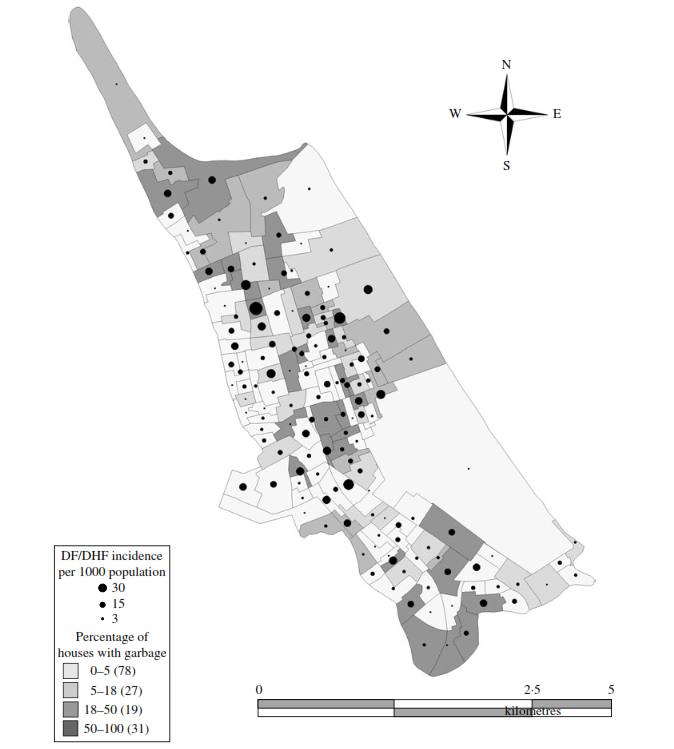
\includegraphics[width=110mm]{./figures/house_with_garbage}
%		\caption{DF/DHF incidence per 1000 population, compared to percentage of houses with poor garbage disposal in Songkhla municipality. Reprinted from \protect\cite{thammapalo2008environmental}.}
%		\label{figure-house_with_garbage}
%	\end{center}
%\end{figure}


% \begin{figure}[htbp]
% \begin{center}
% 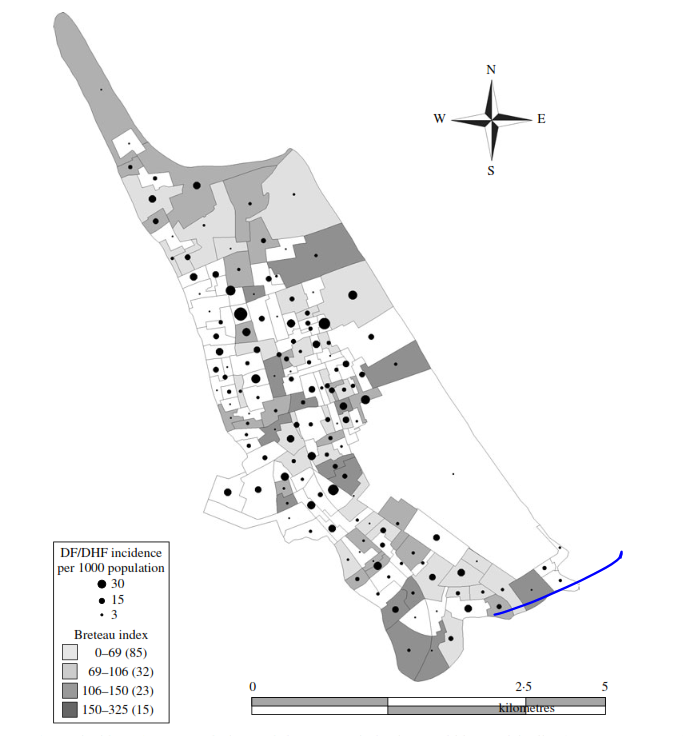
\includegraphics[width=110mm]{./figures/breteau_index}
% \caption{ DF/DHF incidence/1000 population rate and the Breteau index in Songkhla municipality. Reprinted from \protect\cite{thammapalo2008environmental}.}
% \label{figure-breteau_index}
% \end{center}
% \end{figure}

% 2.3.3
\subsection{Near real-time characterization of urban environments: a holistic approach for monitoring dengue fever risk areas: A city of Phitsanulok Province, Thailand}

\cite{sarfraz2014near} extract land-use types using object-based and spatial metric approaches to explore dengue incidence in relation to the surrounding environment in near real-time using Google and Advanced Land Observation Satellite images. Geospatial analysis on public health data indicated that most of the dengue cases were found in densely populated areas \textit{surrounded by dense vegetation}. Dense vegetation can facilitate the invasion of Aedes mosquitoes by providing abundant resting sites. 

%Figure \ref{figure-gps_map_den_cases} shows the incidence of dengue cases in the city of Phitsanulok in 2010 in relation to important landmarks, for example, a hospital, market, temple and school. A positive relationship between dengue cases and neighborhoods was observed based on proximity and spatial analysis. \textit{Proximity analysis} indicated that most of the dengue cases were around \textit{institutions (40\%), religious places (18\%), and markets (15\%)}. The study also reports that dengue incidence was more prevalent in people of 5-24 years of age (67\%), while in terms of occupation, mostly \textit{students, the unemployed, laborers, and farmers (88\%)} were affected.
%
%
%\begin{figure}[htbp]
%	\begin{center}
%		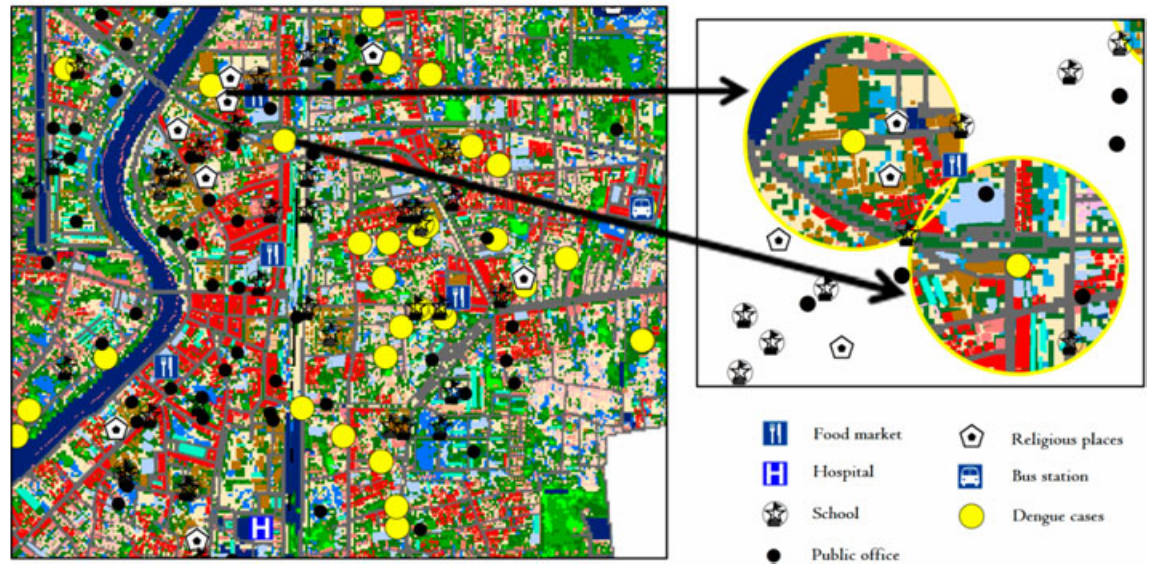
\includegraphics[width=110mm]{./figures/gps_map_den_cases}
%		\caption{ Location of dengue cases (yellow points) in Phitsanulok study area overlaid onto the land-use/land-
%			cover map. Reprinted from \protect\cite{sarfraz2014near}.}
%		\label{figure-gps_map_den_cases}
%	\end{center}
%\end{figure}

% 2.3.4
%\subsection{An information value based analysis of physical and climatic factors affecting dengue fever and dengue haemorrhagic fever incidence: Sukhothai province, Thailand.}
%\label{subsection-regressions-paper}

\cite{nakhapakorn2005information} explores empirical relationship of climatic factors rainfall, temperature and humidity with the DF/DHF incidences using multivariate regression analysis. Sukhothai province located in the northern Thailand, was selected as the study area for this work.  The province has a population of about 521,219. Climate of this area is subtropical with extreme high temperatures rising to 42$^{\circ}$C in April and dipping low up to 13.2$^{\circ}$C in December. Medical data were collected from the Provincial Health Office, Thailand, which collects monthly district level data.  

The purpose of the multiple regressions was to learn more about the relationship between several independent or predictor variables and the dependent or criterion variable (number of DF/DHF cases). 
In general, multiple regression procedures estimate a linear equation of the form:

\begin{equation}
\label{eq:linear}
Y\ =   (B\textsubscript{\textit{0}}) + (B\textsubscript{\textit{1}})(X\textsubscript{\textit{1}}) + (B\textsubscript{\textit{2}})(X\textsubscript{\textit{2}}) + ... + (B\textsubscript{\textit{k}})(X\textsubscript{\textit{k}}) 
\end{equation}

Where k is the number of predictors. Rainfall (R), temperature (T), and relative humidity (H) were considered as the independent variables. There are many related studies also conclude that climate is related to dengue outbreak \cite{li1985rainfall,hales2002potential,rueda1990temperature,tun2000effects,brady2013modelling}. The realtime at time T relationship (ER) between number of DF/DHF cases and the climatic data  (T\textsubscript{\textit{t}}, R\textsubscript{\textit{t}} and H\textsubscript{\textit{t}} ) at time \textit{t} during 5 years is listed in ER-1, ER-2, and ER-3 equations. Multiple regression analysis is employed to develop an empirical model to predict the dengue incidences by using the occurrence of DF/DHF cases and monthly climatic data of 5 years (1997$-$2001).

%\begin{figure}[htbp]
%	\begin{center}
%		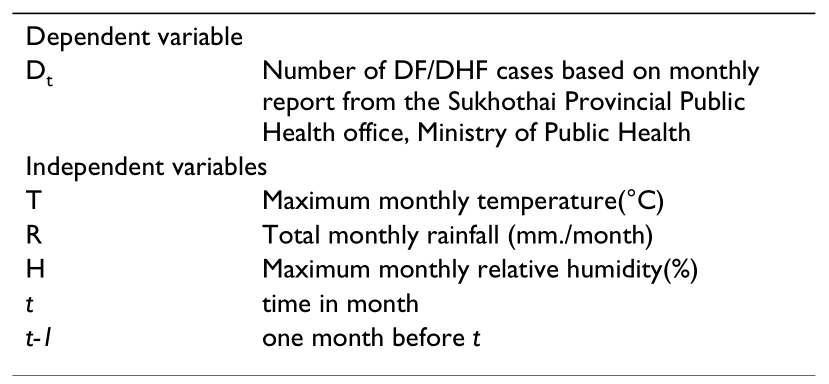
\includegraphics[width=110mm]{./figures/variable}
%		\caption{ Variables in the Sukhothai DF/DHF multiple regression study. Reprinted from \protect\cite{nakhapakorn2005information}.}
%		\label{figure-variable}
%	\end{center}
%\end{figure}

\textbf{ER-1 equation:} 
\begin{equation}
\label{eq:er-1}
D\textsubscript{\textit{t}} =   1408.318 + 0.151(R\textsubscript{\textit{t}}) - 4.368(T\textsubscript{\textit{t}})-12.798(H\textsubscript{\textit{t}} )
\end{equation}

The coefficient of determination ($R^2$) of ER-1 was 0.43.
Multiple regression analysis was carried out for the occurrence of DF/DHF cases for the rainy season.

\textbf{ER-2 equation:} 
\begin{equation}
\label{eq:er-2}
D\textsubscript{\textit{t}} =   -13.893 + 0.377(R\textsubscript{\textit{t}}) + 1.3444(T\textsubscript{\textit{t}}) - 0.276(H\textsubscript{\textit{t}} )
\end{equation}
The coefficient of determination ($R^2$) of ER-2 was 0.62.

According to the development period from a mosquito egg to the human disease, there is a time lag of about one month that leads to DF/DHF cases occurring in 7 - 45 days. The duration of larvae stages is 7 to 12 days, and the lifespan of the female mosquito is about 8 to 15 days. In the meantime, the virus develops in the mosquito for a period of 8$–$10 days. By the time a person infected with dengue virus develops fever, the infection is usually widely disseminated to many people. The virus is found in serum or plasma, in circulating blood cells and in selected tissues, especially those of the immune system, for approximately 2–7 days, roughly corresponding to the period of fever. Thus, DF/DHF cases at time t (in month e.g. May) depend on others factors at time t-1 (i.e. one month before month).

The Empirical Relationship-3 (ER-3) with a one-month time lag as shown below offered a coefficient of determination ($R^2$) as 0.81. Therefore, the ER-3 was selected to model the DF/DHF incidence in Sukhothai as the closest output to the actual data during rainy season and the results were validated with 1998 data, as shown in Figure \ref{figure-er_3}.

\textbf{ER-3 equation:} 
\begin{equation}
\label{eq:er-3}
D\textsubscript{\textit{t}} =   621.824 + 0.345(R\textsubscript{\textit{t-1}}) - 0.609(T\textsubscript{\textit{t-1}}) - 6.321(H\textsubscript{\textit{t-1}} )
\end{equation}

%\begin{figure}[htbp]
%	\begin{center}
%		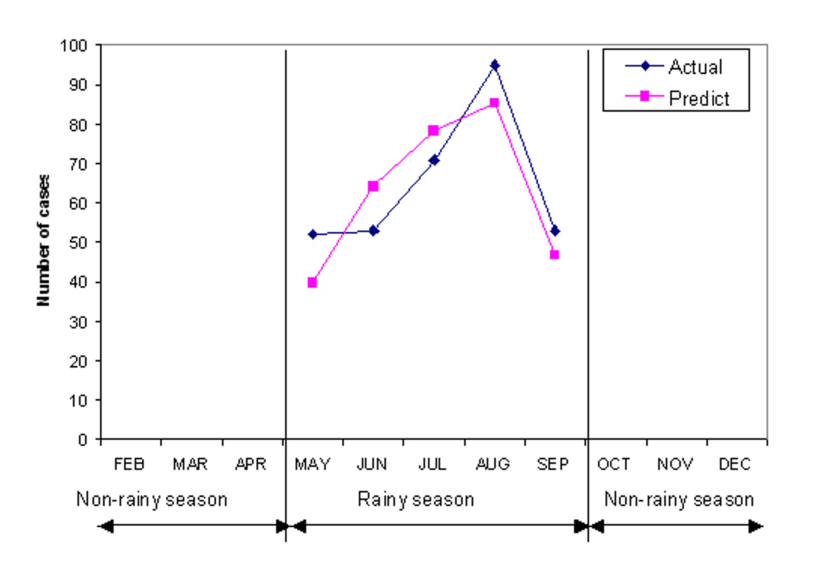
\includegraphics[width=110mm]{./figures/er_3}
%		\caption{ The relationship between actual and forecasted DF/DHF cases in Sukhothai, Thailand in 1998 during rainy season using ER-3. Reprinted from \protect\cite{nakhapakorn2005information}.}
%		\label{figure-er_3}
%	\end{center}
%\end{figure}

% 2.3.5
\subsection{Impact of daily temperature fluctuations on dengue virus transmission by Aedes aegypti.}

The diurnal temperature range (DTR) is the difference between the daily maximum and minimum temperature. \cite{lambrechts2011impact} show that DTR affects two important parameters underlying dengue virus (DENV) transmission by Aedes mosquito.

They evaluated experimentally the effect of DTR on the potential for DENV transmission by Aedes mosquito females under three temperature. Each experiment had the same average temperature (26 °C), but a different amplitude of daily temperature variation; control (DTR = 0$^{\circ}$C), moderate (DTR = 10$^{\circ}$C), and large (DTR = 20$^{\circ}$C). In two independent experiments using different DENV serotypes (DENV-1 and DENV-2), mosquitoes were less susceptible to virus infection and died faster under larger DTR (20$^{\circ}$C).  A thermodynamic model predicted that at mean temperatures <18 $^{\circ}$C, DENV transmission increases as DTR increases, whereas at mean temperatures >18 $^{\circ}$C, larger DTR reduces DENV transmission.

Infection analysis is divided in to two experiments. In the first experiment, rates of infection by a DENV-2 isolate were measured in a total of 525 Aedes mosquito females (175 in each of the three temperature regimes). Result of the first experiment is 97.1\%, 94.9\%, and 78.9\% of females were DENV-2 infected under DTRs of 0 °C, 10 °C, and 20 °C, respectively. In the second experiment, rates of infection by a DENV-1 isolate were measured in 227 Aedes mosquito females (132 in each of the two temperature regimes: low and large DTR regime) Result of the second experiment is, 97.0\% and 88.4\% of females were DENV-1 infected under DTRs of 0 °C and 20 °C, respectively.

Survival analysis is also divided in to two experiments. A total of 900 Aedes mosquito females were included in survival analysis in the first experiment with DENV-2, which 244 died during the course of the experiment. Mean survival times were 27.6, 27.9, and 27.3 days post infection under DTRs of 0 °C, 10 °C, and 20 °C, respectively. Although mean survival times were similar across DTR regimes, only ∼30\% of females under the DTR of 20$^{\circ}$C survived to the end of the experiment, compared with 50\% and ∼70\% under a DTR of 10$^{\circ}$C and 0$^{\circ}$C, respectively. 

%Survival results of the first experiment were confirmed in the second experiment with DENV-1. A total of 317 Aedes mosquito females were included in survival analysis, which 85 died during the course of the experiment. Mean survival times were 28.5 and 22.2 dpi under DTRs of 0 °C and 20 °C, respectively. This experiment conclude that DTR had a statistically significant influence on survival rates as shown in Figure \ref{figure-survive}.
%
%\begin{figure}[htbp]
%	\begin{center}
%		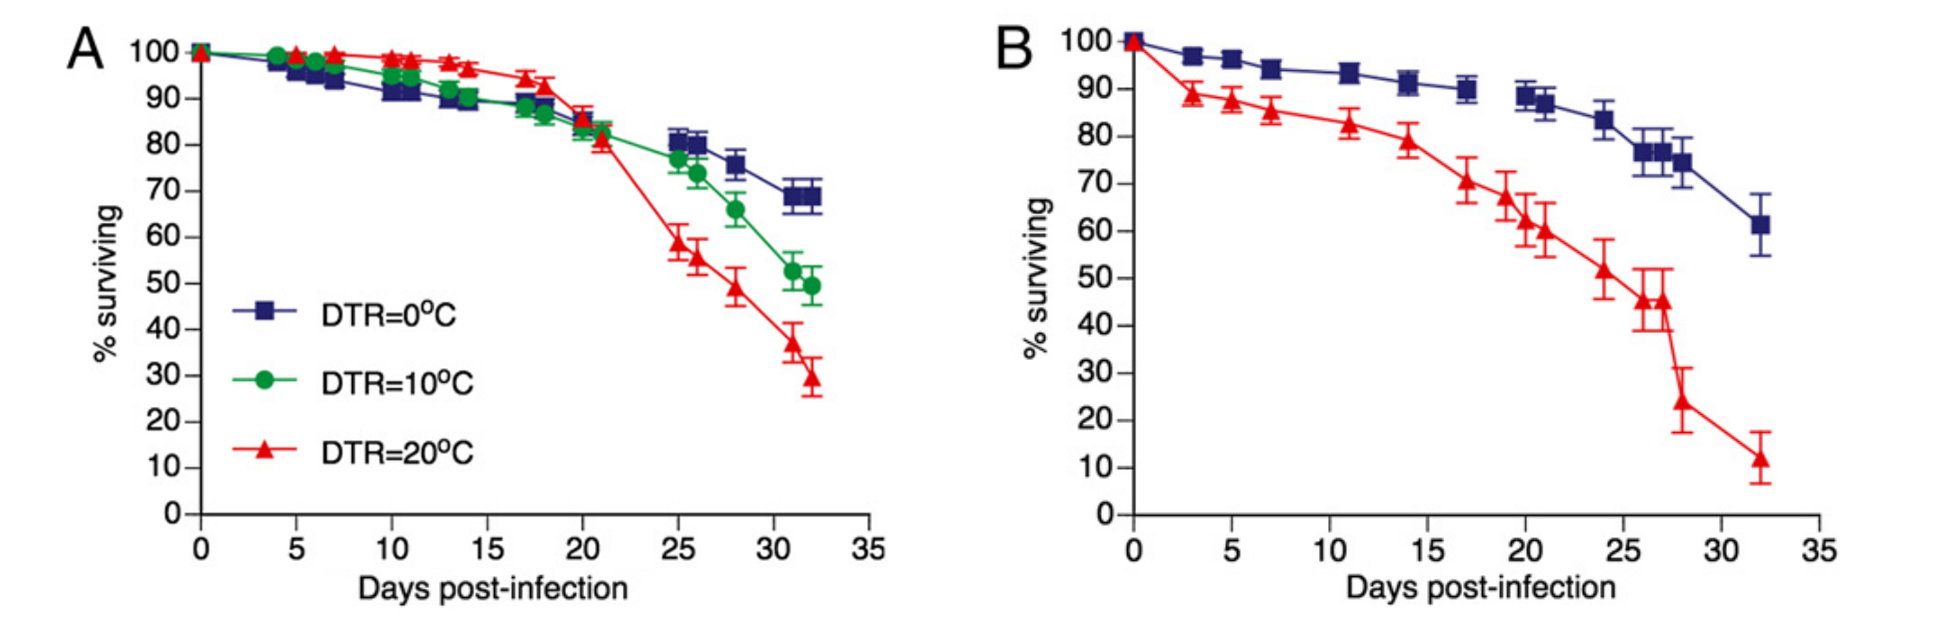
\includegraphics[width=150mm]{./figures/survive}
%		\caption[Effect of DTR on experimental survival of Aedes mosquito females after infected to DENV, Reprinted from \protect\cite{lambrechts2011impact}.]{ Effect of DTR on experimental survival of Aedes mosquito females after infected to DENV. 
%			In A, mosquitoes were exposed to a DENV-2 isolate. Survival curves are significantly different according to log-rank tests (overall: P < 0.0001; DTR = 0$^{\circ}$C vs. DTR = 10$^{\circ}$C: P = 0.0249; DTR = 10$^{\circ}$C vs. DTR = 20$^{\circ}$C: P = 0.0068). In B, mosquitoes were exposed to a DENV-1 isolate. Survival curves are significantly different according to a log-rank test (P < 0.0001). Reprinted from \protect\cite{lambrechts2011impact}.}
%		\label{figure-survive}
%	\end{center}
%\end{figure}


































\section{Methodology}



\subsection{Study area}
\label{section-study-area}



The dengue outbreak in Bangkok can affect to dengue situation for the whole country, because Bangkok is a very crowded city  locate at the center part of Thailand. In the 2010 census, Bangkok had a population of 8.28 million, although just 5.7 million were registered residents. Much of the daytime population commutes from surrounding areas in the region, bringing the total population to 15 million \cite{WPR2015}. During winter season, temperature in Bangkok still high around 28-35 degree Celsius and there is rain in every season \cite {wwo2012}. Figures \ref{figure-avg_temp_bangkok} and \ref{figure-avg_rain_bangkok} show the average temperature and rain of the Bangkok. This makes the city is very suitable for Aedes mosquito to breeding making dengue virus spread from  Bangkok in every season. Moreover, many people who live in Bangkok travel to other provinces frequently, so these people may be the main carriers and multipliers of the virus that cause dengue outbreak in other part of Thailand. 

\begin{figure}[htbp]
	\begin{center}
		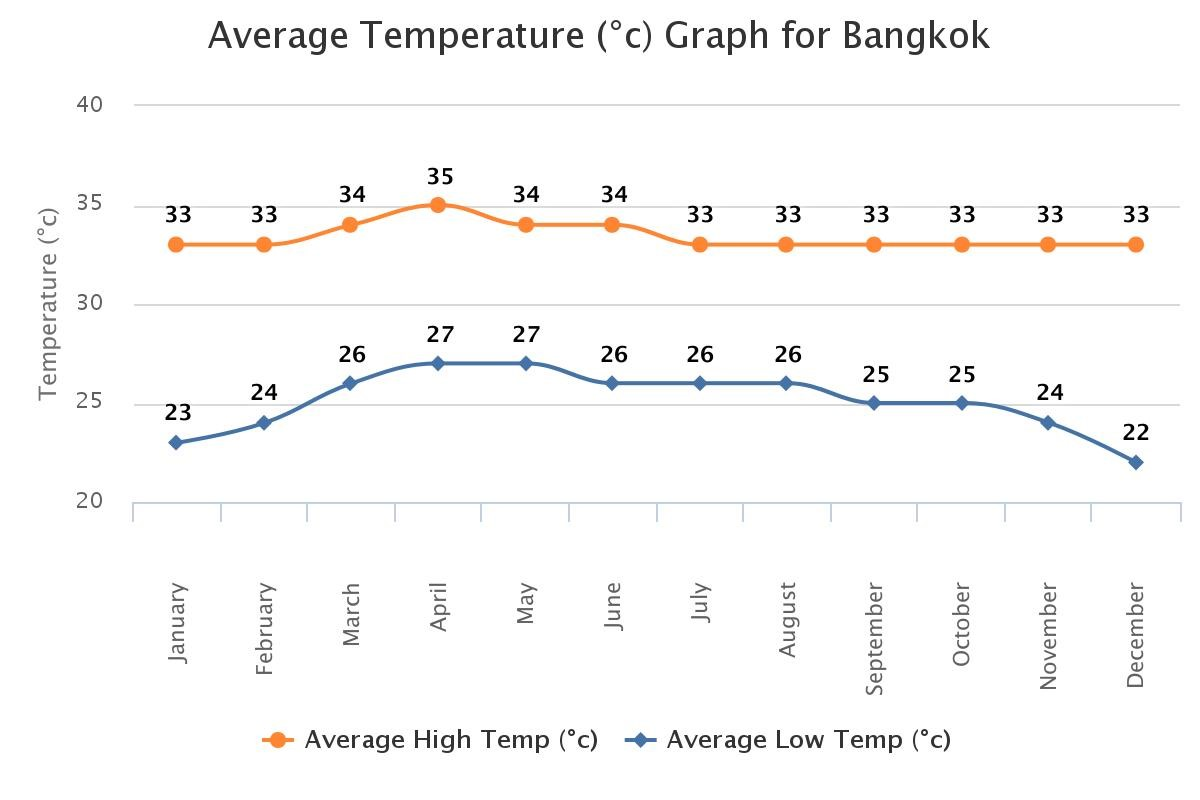
\includegraphics[width=145mm]{./figures/avg_temp_bangkok}
		\caption{Average high and low temperature in Bangkok from 2000-2012. Reprinted from \protect\cite{wwo2012}.}
		\label{figure-avg_temp_bangkok}
	\end{center}
\end{figure}

\begin{figure}[htbp]
	\begin{center}
		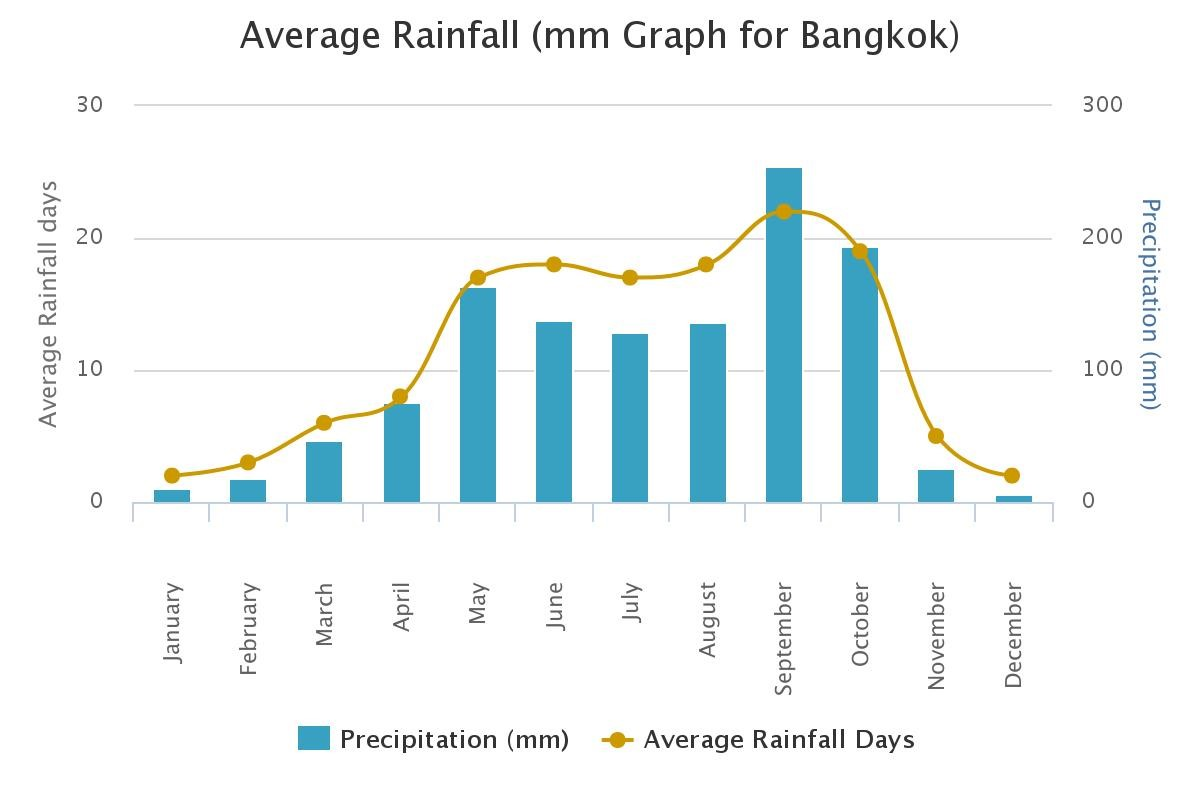
\includegraphics[width=145mm]{./figures/avg_rain_bangkok}
		\caption{Average rainfall in Bangkok from 2000-2012. Reprinted from \protect\cite{wwo2012}.}
		\label{figure-avg_rain_bangkok}
	\end{center}
\end{figure}

Figure \ref{figure-dengue_incident_rate} shows the relationship between incidences of dengue per one hundred thousand people in Thailand versus Bangkok. The dengue incident rate in Bangkok is nearly the same as the whole country. So, if we could reduce dengue incident rates in Bangkok, the rate in Thailand will be reduce too because there will be fewer dengue carriers who travel from Bangkok to other parts of Thailand.

\begin{figure}[htbp]
	\begin{center}
		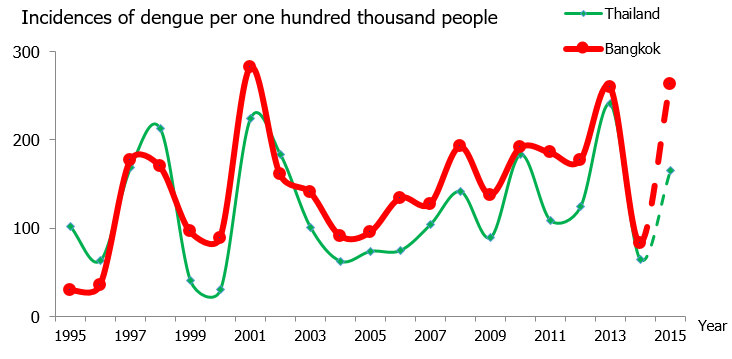
\includegraphics[width=140mm]{./figures/dengue_incident_rate}
		\caption{ Relationship between incidences of dengue per one hundred thousand people in Thailand versus Bangkok from 2005 - 2014.}
		\label{figure-dengue_incident_rate}
	\end{center}
\end{figure}

% 3.1.1
\subsection{Bangkok districts}

The Bangkok city covers an area of 1,568.737 square kilometres and it is subdivided into 50 districts , which are further subdivided into 169 sub-districts. Total population who registered in Bangkok is 5,693,884 and more than three million people are live in Bangkok without registered. Table \ref{table-bangkok-district} and figure \ref{figure-bangkok_district} show district name, map and population statistic in each area. The average registered population of Bangkok districts in 2014 is 113845. The highest population district is Saimai (194,511) and the lowest population district is Samphanthawongse (26359). But the highest and lowest population density district are Phranakhon (157791 men/km 2) and Thawiwatthana (2948 men/km 2).  Data of Bangkok statistics described more later in subsection "Prediction variable".

\begin{table}[htbp]
	\centering
	\scriptsize
	\label{table-bangkok-district}
	\resizebox{1.2\textwidth}{!}{
	\begin{tabular}{|l|l|l|l|l|}
		\hline
		ID Map & District Name & Population & Area  & Density\\
		\hline
		1 & Phranakhon & 55373 & 5.536 & 157791\\
		\hline
		2 & Bangbon & 107140 & 34.745 & 3084\\
		\hline
		3 & Chomthong & 156030 & 26.265 & 28111\\
		\hline
		4 & Bangrak & 46472 & 5.536 & 42529\\
		\hline
		5 & Bangkhae & 191966 & 44.456 & 18428\\
		\hline
		6 & Bangkapi & 148964 & 28.523 & 10853\\
		\hline
		7 & Patumwan & 51557 & 8.369 & 28172\\
		\hline
		8 & Pom prap & 49280 & 1.931 & 127030\\
		\hline
		9 & Prakanong & 92448 & 13.986 & 6610\\
		\hline
		10 & Minburi & 139771 & 63.645 & 4619\\
		\hline
		11 & Don muang & 168197 & 36.803 & 14759\\
		\hline
		12 & Yannawa & 80843 & 16.662 & 9651\\
		\hline
		13 & Samphanthawongse & 26359 & 1.416 & 55837\\
		\hline
		14 & Payathai & 72203 & 9.595 & 7525\\
		\hline
		15 & Thung khru & 119349 & 30.741 & 7861\\
		\hline
		16 & Bangkok yai & 70003 & 6.18 & 27711\\
		\hline
		17 & Huai khwang & 80002 & 15.033 & 16746\\
		\hline
		18 & Thawiwatthana & 77121 & 50.219 & 2948\\
		\hline
		19 & Taling chan & 105857 & 29.479 & 26455\\
		\hline
		20 & Suanluang & 118371 & 23.678 & 4999\\
		\hline
		21 & Lat Krabang  & 168309 & 123.859 & 10304\\
		\hline
		22 & Dindaeng & 127260 & 8.354 & 15233\\
		\hline
		23 & Nongkhaem & 153175 & 35.825 & 8572\\
		\hline
		24 & Radburana & 84881 & 15.782 & 10678\\
		\hline
		25 & Bangplad & 96787 & 11.36 & 34173\\
		\hline
		26 & Bangsue & 128995 & 11.545 & 22359\\
		\hline
		27 & Bung kum & 145514 & 24.311 & 17772\\
		\hline
		28 & Watthana & 83520 & 12.565 & 18145\\
		\hline
		29 & Pasricharoen & 129238 & 17.834 & 51163\\
		\hline
		30 & Prawet & 166364 & 52.49 & 9346\\
		\hline
		31 & Saphansung & 92735 & 28.124 & 3297\\
		\hline
		32 & Nong chokn & 162598 & 236.261 & 5799\\
		\hline
		33 & Klongtoey & 107221 & 12.994 & 22270\\
		\hline
		34 & Thon buri & 115330 & 8.551 & 98020\\
		\hline
		35 & Jatujak & 160366 & 32.908 & 26676\\
		\hline
		36 & Bangkuntien & 173144 & 120.687 & 3940\\
		\hline
		37 & Ratchathervi & 73790 & 7.126 & 41593\\
		\hline
		38 & Lat Phrao & 122196 & 22.157 & 10180\\
		\hline
		39 & Sathorn & 82432 & 9.326 & 28089\\
		\hline
		40 & Saimai & 194511 & 44.615 & 13386\\
		\hline
		41 & Laksi & 107797 & 22.841 & 9472\\
		\hline
		42 & Bangkhen & 190659 & 42.123 & 9221\\
		\hline
		43 & Kannayao & 92094 & 25.98 & 7086\\
		\hline
		44 & Bang kholam & 92273 & 10.921 & 28042\\
		\hline
		45 & Wang thonglang & 114245 & 19.265 & 24568\\
		\hline
		46 & Klongsamwa & 178958 & 110.686 & 8751\\
		\hline
		47 & Bangna & 94315 & 18.789 & 5020\\
		\hline
		48 & Klongsan & 75224 & 6.051 & 54926\\
		\hline
		49 & Bangkok noi & 116653 & 11.944 & 52187\\
		\hline
		50 & Dusit & 104394 & 10.665 & 58514\\
		\hline
	\end{tabular}
}
	\caption{Bangkok district population in 2014. Density is number of people per km$^{2}$. Data from Department of Provincial Administration, Ministry of Interior, Thailand }
\end{table}



\begin{figure}[htbp]
	\begin{center}
		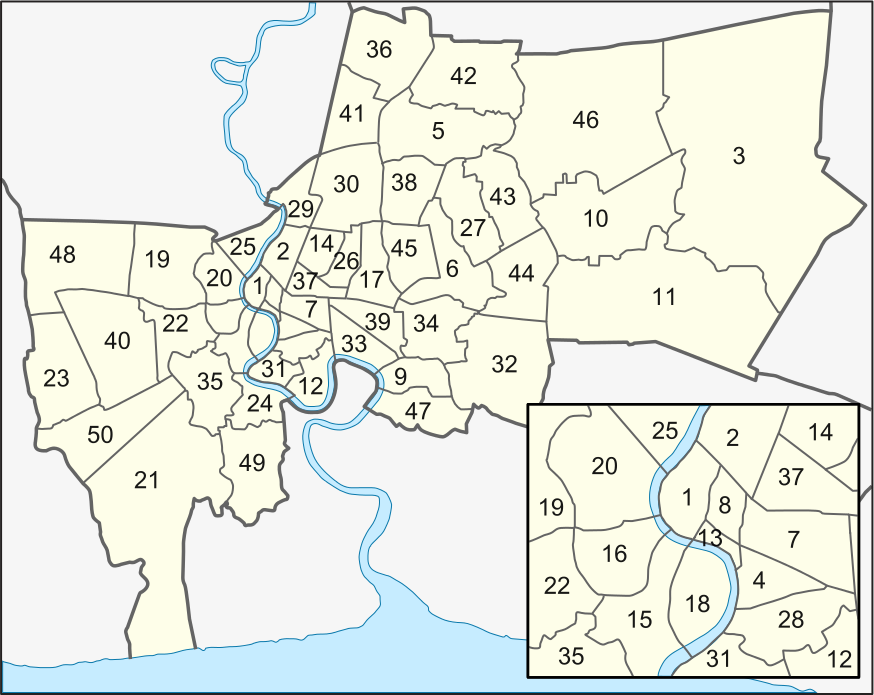
\includegraphics[width=140mm]{./figures/bangkok_district}
		\caption{ Bangkok districts, Reprinted from \protect\cite{wikibangkok}.}
		\label{figure-bangkok_district}
	\end{center}
\end{figure}

% 3.1.2
\subsection{Dengue fever in Bangkok district}


Figure \ref{figure-bangkok-data} (a) shows the increase of dengue cases in Bangkok up to 2015. The average number of dengue cases in Bangkok from 2005 until 2015 is around 10,758 cases per year. The highest number of dengue cases in Bangkok is 28,177 cases which happened in 2015. Figure \ref{figure-bangkok-data} (b) shows changes in dengue serotypes from 2005 to 2015. The percentage of dengue serotypes DENV 1 - 4 in the central part of Thailand changed every year, making people who already have immunity to one serotype susceptible to infection with another serotype in the following year. Figure \ref{figure-dengue_bangkok_2015} shows the effect of season on dengue cases. In rain season (mid May - October), dengue cases rise dramatically, and then they decrease suddenly in summer season (February - mid May). The reason that November has the highest number cases is that dengue virus in patients need 4 - 10 days for the incubation period. So most dengue patients in November are infected in rain season (October).  


\begin{figure}[htbp]
	\begin{center}
		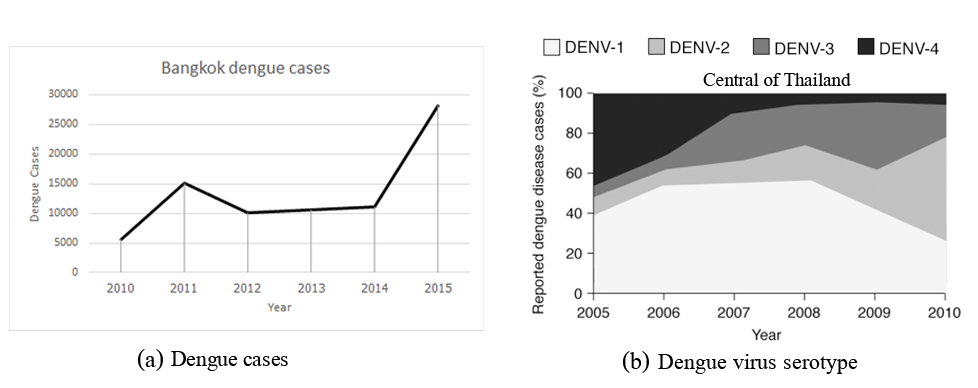
\includegraphics[width=145mm]{./figures/bangkok_dengue_data}
		\caption{ (a) Dengue cases from 2010 - 2015 in Bangkok. (b) Dengue serotypes from 2005 - 2010 in central Thailand. Data from Department of Disease Control 13th Division and \protect\cite{limkittikul2014epidemiological}. }
		\label{figure-bangkok-data}
	\end{center}
\end{figure}


\begin{figure}[htbp]
	\begin{center}
		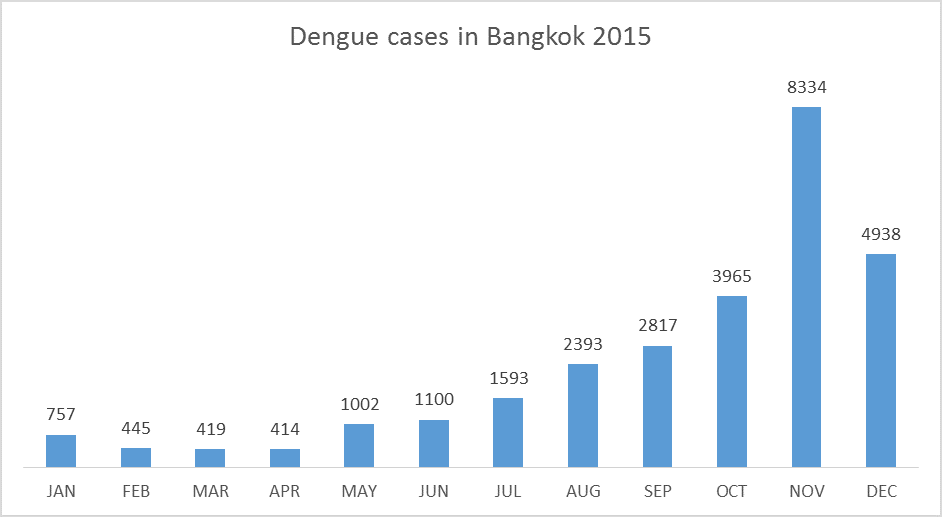
\includegraphics[width=120mm]{./figures/dengue_bangkok_2015}
		\caption{ Monthly dengue cases in Bangkok  2015. Data from Department of Disease Control 13th Division. }
		\label{figure-dengue_bangkok_2015}
	\end{center}
\end{figure}














\subsection{Prediction variable and data collection}
\label{section-Prediction-variable}

According to Dr Sonpon and Dr Nicholas, there are three main factors that affect to dengue incidence cases: other cases of dengue virus, presence of Aedes mosquitoes, and various human factors. Dengue fever cannot spread to humans from other animal; mosquitoes are mainly carries. Typically, people infected with dengue virus are asymptomatic (80\%) or have only mild symptoms , such as an uncomplicated fever \cite{whitehorn2010dengue,reiter2010yellow}. In Bangkok's case, dengue fever and dengue hemorrhagic fever were reported in each season,  mean, dengue virus  is always present in human too. Once infected, \textit{humans} become the main carriers and multipliers of the virus, serving as a source of the virus for uninfected \textit{Aedes mosquitoes} to carry. All prediction variables that I choose are related to these three main factors. 

\subsubsection{Dengue virus prediction variable}

I selected 2 prediction variables related to dengue virus factors: 

\begin{enumerate}
	% 	\item \textbf{Monthly DF/DHF cases in district} represents amount of dengue virus in target district. 
	% 
	% 	\item \textbf{Monthly DF/DHF cases in connected districts} represents amount of dengue virus that may affect to target district
	
	\item \textbf{Monthly DF/DHF incidents in the district} represents the number of dengue virus report in the target district. 
	
	\item \textbf{Monthly DF/DHF incident in the nearby districts} represents the number of dengue virus reports which may affect to the target district
	
\end{enumerate}

All DF/DHF case data are provided by the Department of Disease Control, Bangkok.


\subsubsection{Aedes mosquito prediction variables}

I selected 2 prediction variables related to the Aedes mosquito factor:

\begin{enumerate}
	\item \textbf{Monthly rainfall in district} represents the density of Aedes mosquitoes in the target district. 
	
	\item \textbf{Monthly average diurnal temperature range (DTR) in Bangkok} represents the health of the dengue virus in Aedes mosquito. Higher DTR means  lower health of dengue virus in Aedes mosquito, deceasing infection rates.
\end{enumerate}

Rainfall data is provided by Department of Drainage and Sewerage, Bangkok ,and temperature data is provided by Meteorological Department, Thailand.


\subsubsection{Human prediction variables}

I selected 3 prediction variable that related to human factor:

\begin{enumerate}
	\item \textbf{Population with age less than 35 in the district} represents the proportion of the district population that has a high risk for dengue fever. 
	
	\item \textbf{Population age 35+ in the district} represents the proportion of the district population that has a low risk for dengue fever.
	
	% 	\item \textbf{Yearly population density in district} represents how easy to transmit dengue virus from one person other other person by Aedes mosquito. 
	
	\item \textbf{Number of communities  in  the district} represents how large the group are, make it more of less convenient transmission of dengue virus by Aedes mosquito.
	
\end{enumerate}

Bureau of Epidemiology, Thailand reports that 80\% of dengue patient from 1993 - 2013 are in the age range between 5 - 35 years old. So I divide the population into two groups: population with age less than or equal to 35 as high risk group and those older than 35 as low risk group. Population and community data are provided by the Department of Social Development, Bangkok. 

I did a basic analysis of dengue case data and human prediction variable in Bangkok in Microsoft Excel. I determined the relationship between average dengue incidence rate  from 2005-2015 and the number of communities in each individual district. Figure \ref{figure-dengue_community_vs_cases} shows that fewer communities district may have higher dengue than district with a large number of communities.


\begin{figure}[htbp]
	\begin{center}
		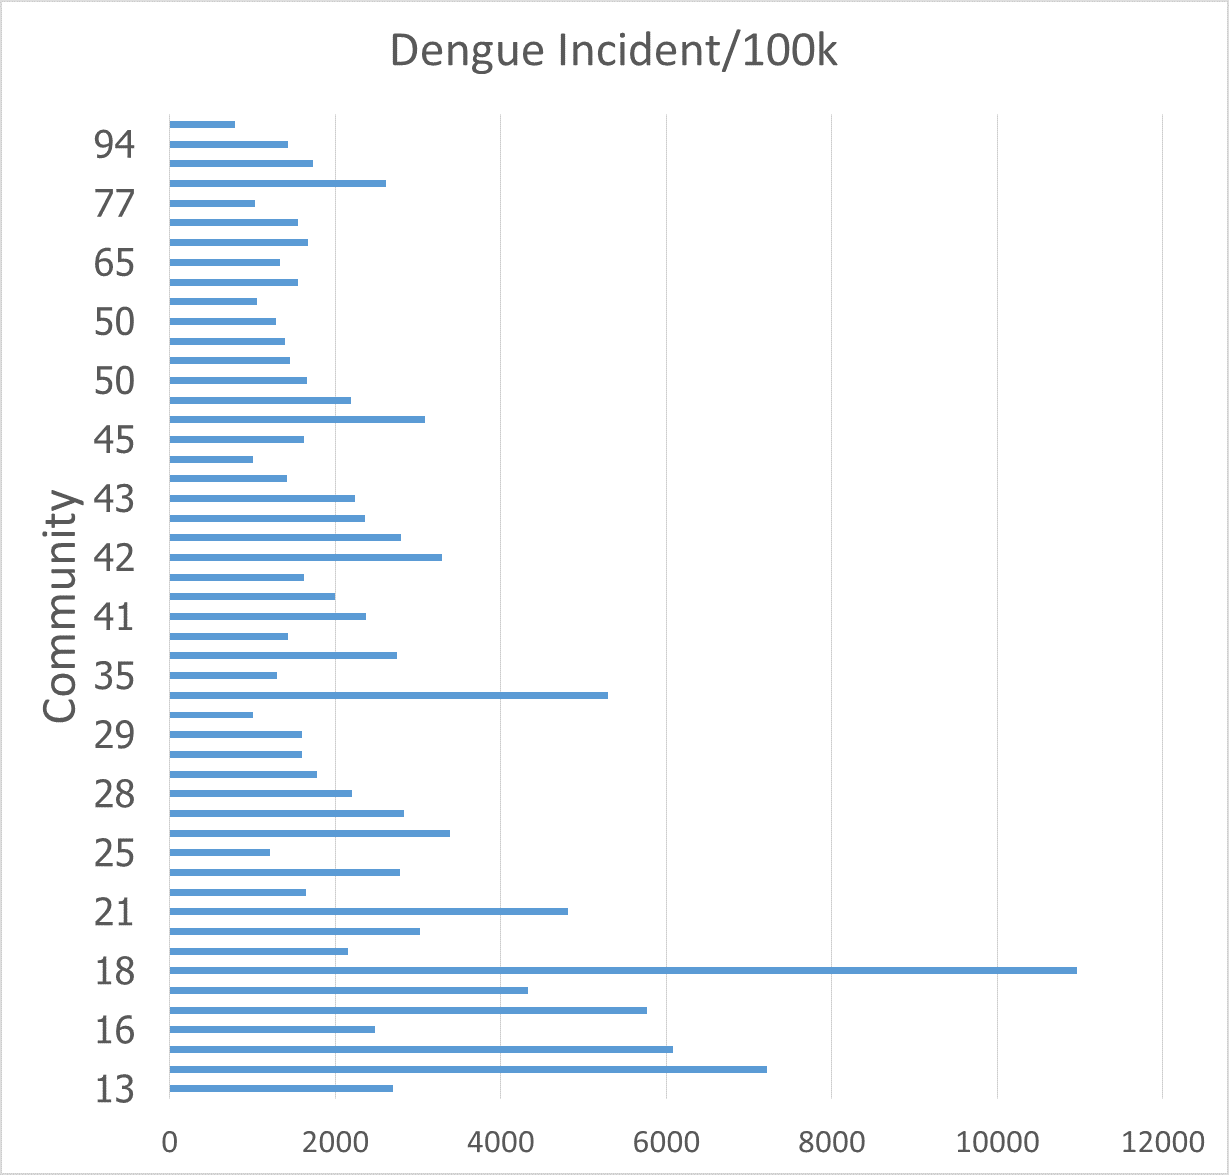
\includegraphics[width=120mm]{./figures/dengue_community_vs_cases}
		\caption{ Average dengue rates per 100,00 people from 2005-2015 and number of communities in individual district of Bangkok.  Dengue cases data from Department of Disease Control 13th division and Community data from Department of Social Development, Bangkok.}
		\label{figure-dengue_community_vs_cases}
	\end{center}
\end{figure}








\subsection{Data preparation and prediction methodology}
\label{section-Prediction-model-method}


\subsubsection{Multiple linear regression model}
\label{section-linear-regression-model}

For the first prediction model in this research, we  will use multiple linear regression.
\textbf{Dengue virus prediction variables}\\ 
MDR\textsubscript{x} = Monthly DF/DHF incident rate in district X \\
MNDR\textsubscript{x} = Monthly DF/DHF incident rate in the Nearby district X\\

\textbf{Aedes mosquito prediction variables}\\
MR\textsubscript{x} = Monthly Rainfall in district X\\
MDTR\textsubscript{b} = Monthly average Diurnal Temperature Range (DTR) in Bangkok\\

\textbf{Human prediction variables}\\
P35\textsubscript{x} = Population who age $\leqslant$ 35 in district X\\
P35+\textsubscript{x} = Population who age $\textgreater$ 35 in district X\\
C\textsubscript{x}  = Number of Communities in district X

\textbf{Prediction model}\\
At first, I begin with predicting dengue incident rate in the next month by using dengue virus prediction variables and Aedes mosquito prediction variables as the inputs of multiple regression model.

DR\textsubscript{x} = DF/DHF incident rate in district X \\
$DR\textsubscript{x} = b\textsubscript{0} + b\textsubscript{1}MDR\textsubscript{x} + b\textsubscript{2}MNDR\textsubscript{x} + b\textsubscript{3}MR\textsubscript{x} + b\textsubscript{4}MDTR\textsubscript{x}$

\textbf{Dengue-Community impact}\\
Then, to calculate dengue$-$community impact, I will use human prediction variable and dengue virus prediction variable of each district from the previous month to calculate the calculate community by using multiple Logistic Regression model.
The community impact will tell the effect of district structure to dengue virus outbreak.

DCI\textsubscript{x} = Dengue$-$community impact in district X \\
$DCI\textsubscript{x} = [1 + exp(\alpha X)]^{-1}  $ \\
$\alpha X = b\textsubscript{0} + b\textsubscript{1}MDR\textsubscript{x} + b\textsubscript{2}C\textsubscript{x}$

\textbf{Immunity estimation}\\
As I described in Section \ref{section-Prediction-variable}, 80\% of people infected with dengue virus are asymptomatic. To approximate how many people have dengue virus immunity,the number of DF/DHF cases must be extrapolated to estimate the actual number of infected people in the target district. 

DC\textsubscript{x} = DF/DHF cases in district X \\
PM\textsubscript{x} = Number of people who immune to dengue virus in district X (people who already infected dengue virus in previous six months )

$PM\textsubscript{x} = DC\textsubscript{x} \times 100\%/20\%$

\textbf{Estimate actual dengue cases}\\
Lastly, I will combine both predictor variables by dividing the population into two groups: the high risk population (age $\leqslant$ 35) and the low risk population (age $\textgreater$ 35). Then I will multiply the result with dengue\-community impact to calculate the DF/DHF cases in the target district.

PH\textsubscript{x} = Population that has a high risk for dengue fever in district X \\
$PH\textsubscript{x} = P35\textsubscript{x} - PM\textsubscript{x} \times 80\%$

PL\textsubscript{x} = Population that has a Low risk for dengue fever in district X \\
$PL\textsubscript{x} = P35+\textsubscript{x} - PM\textsubscript{x} \times 20\%$

$DC\textsubscript{x} = (1 + DCI\textsubscript{x}) \times ((80\% \times DR\textsubscript{x}) \times PH\textsubscript{x} + (20\% \times DR\textsubscript{x}) \times PL\textsubscript{x})$

To evaluate the prediction model, I will compare the result (DF/DHF cases in the target district) with prediction model that use only DF/DHF cases to predict and also compare it with the actual dengue cases. 


\begin{figure}[htbp]
	\begin{center}
		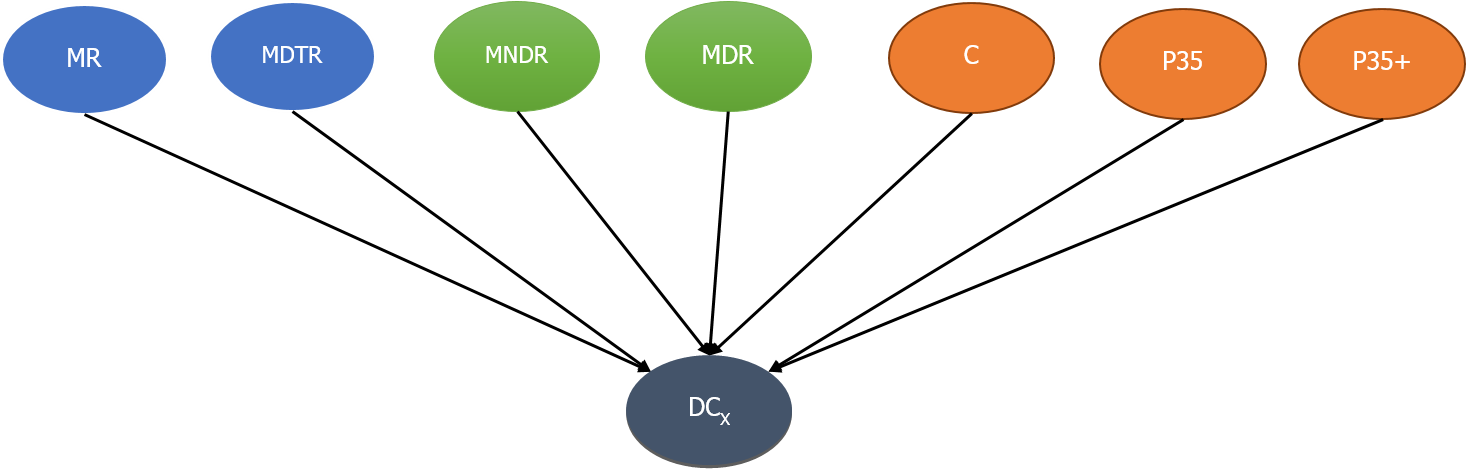
\includegraphics[width=120mm]{./figures/regression_dengue}
		\caption{Multiple regression model of dengue outbreak prediction.}
		\label{figure-regression_dengue}
	\end{center}
\end{figure}

\subsubsection{Multiple logistic regression model}
\label{section-Logistic-regression-model}

As a second model for comparison I will use a multiple logistic regression model to predict the probability that dengue virus will outbreak in the target district. This model will help to warn official in districts outbreaks tend to occur in next month. Based on the prediction, the public health officer and citizen in the district can prepare themselves.

This model will use the same input variable as \ref{section-linear-regression-model}

\textbf{Estimate percentage of people who infected dengue virus}\\

DOS\textsubscript{x} = Dengue Outbreak status in district X (Percentage of population infected, 0 = None, 1 = 100\% infected)

$DOS\textsubscript{x} =  [1 + exp(\beta X)]^{-1}  $ \\
$\beta X =   b\textsubscript{0} + b\textsubscript{1}MDR\textsubscript{x} + b\textsubscript{2}MNDR\textsubscript{x} + b\textsubscript{3}MR\textsubscript{x} + b\textsubscript{4}MDTR\textsubscript{x}$

\begin{figure}[htbp]
	\begin{center}
		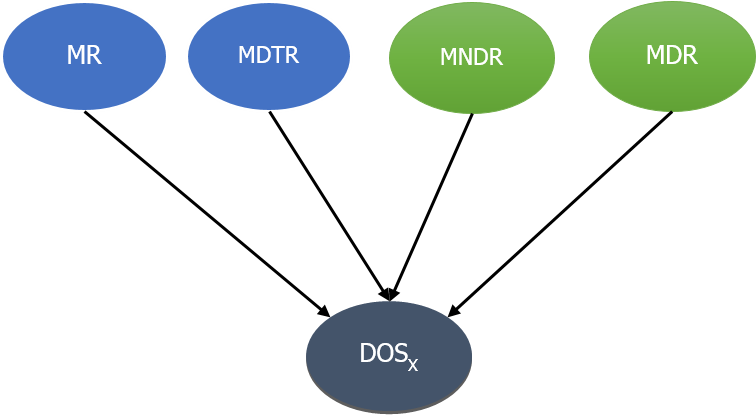
\includegraphics[width=120mm]{./figures/logistic_dengue}
		\caption{Multiple Logistic Regression model of dengue outbreak prediction.}
		\label{figure-logistic_dengue}
	\end{center}
\end{figure}

\subsubsection{Bayesian network model}
\label{section-bayesian-network-model}

The are many variables in the Bayesian network model that I designed DF/DHF incident rate prediction based on my literature reviews and expert interviews. I divide the Bayesian network into 2 parts.

The first part is a Bayesian network model to predict mosquito density in the target area. There are three categories of mosquito density: Low, Moderate, and High. I believe this variable can be predicted from “density of outdoor likely breeding spots”, “density of indoor likely breeding spots” and “diurnal temperature range”. Figure \ref{figure-bn_mosquito_density} depicts the directed acyclic graph for the Bayesian network, and table \ref{table-bn-md-cpd} describes the conditional probability distributions of variables in model.

\begin{figure}[htbp]
	\begin{center}
		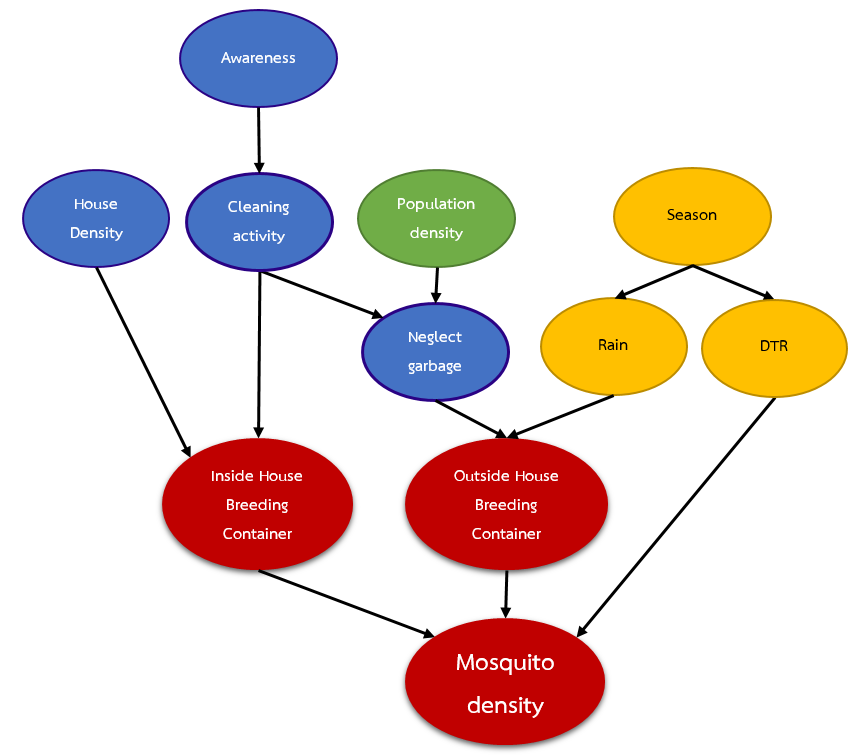
\includegraphics[width=150mm]{./figures/bn_mosquito_density}
		\caption{Directed acyclic graph of Mosquito density Bayesian network model}
		\label{figure-bn_mosquito_density}
	\end{center}
\end{figure}

%\begin{table}[htbp]
%	\label{table-bn-md-dag}
%	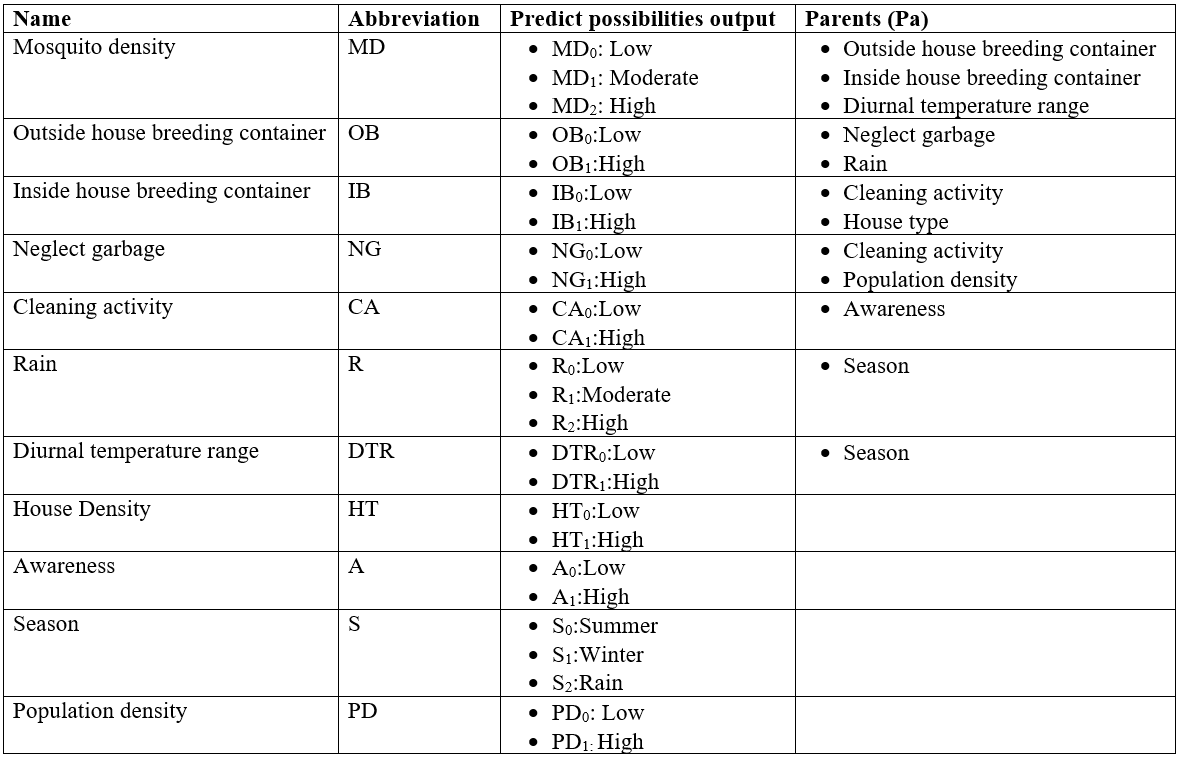
\includegraphics[width=150mm]{./figures/bn_md_dag}
%	\caption{Value of each variables in Mosquito density Bayesian network model}
%\end{table}


	\begin{table}[!htbp]
		\centering
		\normalsize
%		\resizebox{1.4\textwidth}{!}
     \resizebox{1.2\textwidth}{!}{
		\begin{tabular}{|l|p{2cm}|l|l|} 
			\hline
			Name & Abbreviation & Predict possibilities output & Parents (Pa)\\
			\hline
			Mosquito density & MD &  $MD_0$: Low &  Outside house breeding container\\
			&  &  $MD_1$: Moderate &  Inside house breeding container\\
			&  &  $MD_2$: High &  Diurnal temperature range\\
			\hline
			Outside house breeding container & OB &  $OB_0$:Low &  Neglect garbage\\
			&  &  $OB_1$:High &  Rain\\
			\hline
			Inside house breeding container & IB &  $IB_0$:Low &  Cleaning activity\\
			&  &  $IB_1$:High &  House type \\
			\hline
			Neglect garbage & NG &  $NG_0$:Low &  Cleaning activity\\
			&  &  $NG_1$:High &  Population density\\
			\hline
			Cleaning activity & CA &  $CA_0$:Low &  Awareness \\
			&  &  $CA_1$:High & \\
			\hline
			Rain & R &  $R_1$:Low &  Season \\
			&  &  $R_1$:Moderate & \\
			&  &  $R_2$:High & \\
			\hline
			Diurnal temperature range & DTR &  $DTR_0$:Low &  Season \\
			&  &  $DTR_1$:High & \\
			\hline
			House Density & HT &  $HT_0$:Low & \\
			&  &  $HT_1$:High & \\
			\hline
			Awareness & A &  $A_0$:Low & \\
			&  &  $A_1$:High & \\
			\hline
			Season & S &  $S_0$:Summer & \\
			&  &  $S_1$:Winter & \\
			&  &  $S_2$:Rain & \\
			\hline
			Population density & PD & $PD_0$:Low & \\
			&  &  $PD_1$:High & \\
			\hline
		\end{tabular}
	}
		\caption{Value of each variables in Mosquito density Bayesian network model}
		\label{table-bn-md-dag}
	\end{table}







%\begin{table}[htbp]
%	\label{table-bn-md-cpd}
%	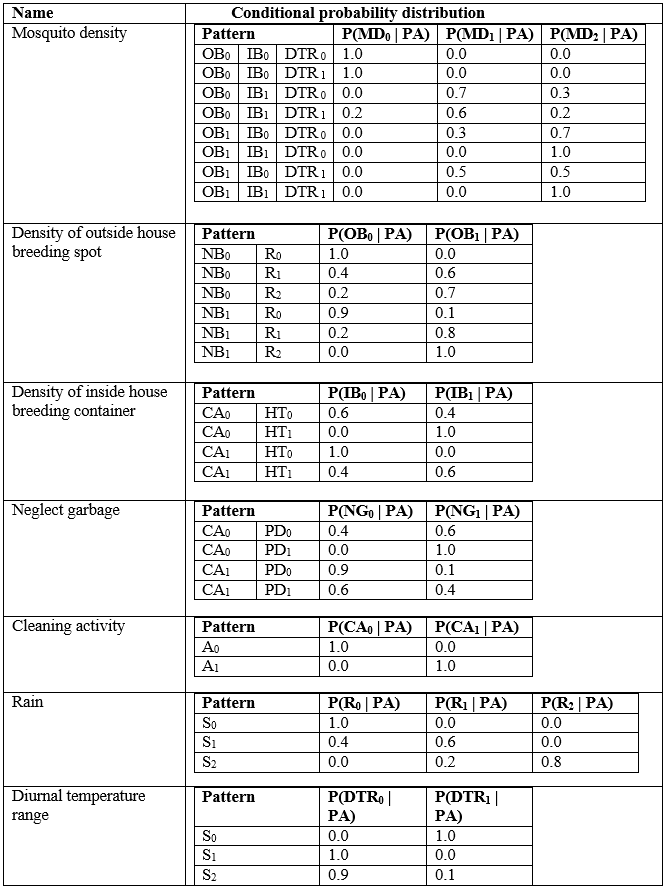
\includegraphics[width=150mm]{./figures/bn_md_cpd}
%	\caption{Conditional probability distribution of each variables in Mosquito density Bayesian network model}
%\end{table}


	
	\begin{table}[!htbp]
		\centering
		\normalsize
		\begin{tabular}{|l|l|l|l|l|l|}
			\hline
			\multicolumn{3}{|l|}{Pattern}	 & P( $MD_0$ $\mid$ PA) & P($MD_1$ $\mid$ PA) & P($MD_2$  $\mid$ PA)\\
			\hline
			$OB_0$ & $IB_0$ & $DTR_0$ & 1 & 0 & 0\\
			\hline
			$OB_0$ & $IB_0$ & $DTR_1$ & 1 & 0 & 0\\
			\hline
			$OB_0$ & $IB_1$ & $DTR_0$ & 0 & 0.7 & 0.3\\
			\hline
			$OB_0$ & $IB_1$ & $DTR_1$ & 0.2 & 0.6 & 0.2\\
			\hline
			$OB_1$ & $IB_0$ & $DTR_0$ & 0 & 0.3 & 0.7\\
			\hline
			$OB_1$ & $IB_1$ & $DTR_0$ & 0 & 0 & 1\\
			\hline
			$OB_1$ & $IB_0$ & $DTR_1$ & 0 & 0.5 & 0.5\\
			\hline
			$OB_1$ & $IB_1$ & $DTR_1$ & 0 & 0 & 1\\
			\hline
		\end{tabular}
		\caption{ Conditional probability distribution of mosquito density}
	\end{table}
	
	
	\begin{table}[!htbp]
		\centering
		\normalsize
		\begin{tabular}{|l|l|l|l|}
			\hline
			\multicolumn{2}{|l|}{Pattern}  & P(OB0 $\mid$ PA) & P(OB1 $\mid$ PA)\\
			\hline
			$NB_0$ & $R_0$ & 1 & 0\\
			\hline
			$NB_0$ & $R_1$ & 0.4 & 0.6\\
			\hline
			$NB_0$ & $R_2$ & 0.2 & 0.7\\
			\hline
			$NB_1$ & $R_0$ & 0.9 & 0.1\\
			\hline
			$NB_1$ & $R_1$ & 0.2 & 0.8\\
			\hline
			$NB_1$ & $R_2$ & 0 & 1\\
			\hline
		\end{tabular}
		\caption{Conditional probability distribution of density of outside house breeding spot}
	\end{table}
	
	\begin{table}[!htbp]
		\centering
		\normalsize
		\begin{tabular}{|l|l|l|l|}
			\hline
			\multicolumn{2}{|l|}{Pattern}  & P(IB0 $\mid$ PA) & P(IB1$\mid$ PA)\\
			\hline
			CA0 & HT0 & 0.6 & 0.4\\
			\hline
			CA0 & HT1 & 0 & 1\\
			\hline
			CA1 & HT0 & 1 & 0\\
			\hline
			CA1 & HT1 & 0.4 & 0.6\\
			\hline
		\end{tabular}
		\caption{Conditional probability distribution of density of inside house breeding container}
	\end{table}
	
	\begin{table}[!htbp]
		\centering
		\normalsize
		\begin{tabular}{|l|l|l|l|}
			\hline
			\multicolumn{2}{|l|}{Pattern}  & P(NG0 $\mid$ PA) & P(NG1 $\mid$ PA)\\
			\hline
			CA0 & PD0 & 0.4 & 0.6\\
			\hline
			CA0 & PD1 & 0 & 1\\
			\hline
			CA1 & PD0 & 0.9 & 0.1\\
			\hline
			CA1 & PD1 & 0.6 & 0.4\\
			\hline
		\end{tabular}
		\caption{Conditional probability distribution of neglect garbage}
	\end{table}
	
	\begin{table}[!htbp]
		\centering
		\normalsize
		\begin{tabular}{|l|l|l|}
			\hline
			Pattern & P(CA0 $\mid$ PA) & P(CA1 $\mid$ PA)\\
			\hline
			A0 & 1 & 0\\
			\hline
			A1 & 0 & 1\\
			\hline
		\end{tabular}
		\caption{Conditional probability distribution of cleaning activity}
	\end{table}
	
	
	\begin{table}[!htbp]
		\centering
		\normalsize
		\begin{tabular}{|l|l|l|l|}
			\hline
			Pattern & P(R0 $\mid$ PA) & P(R1 $\mid$ PA) & P(R2 $\mid$ PA)\\
			\hline
			S0 & 1 & 0 & 0\\
			\hline
			S1 & 0.4 & 0.6 & 0\\
			\hline
			S2 & 0 & 0.2 & 0.8\\
			\hline
		\end{tabular}
		\caption{Conditional probability distribution of rain}
	\end{table}
	
	\begin{table}[!htbp]
		\centering
		\normalsize
		\begin{tabular}{|l|l|l|}
			\hline
			Pattern & P(DTR0 $\mid$  PA) & P(DTR1 $\mid$  PA)\\
			\hline
			S0 & 0 & 1\\
			\hline
			S1 & 1 & 0\\
			\hline
			S2 & 0.9 & 0.1\\
			\hline
		\end{tabular}
		\caption{Conditional probability distribution of Diurnal temperature range}
	\end{table}
	
	\begin{table}[!htbp]
		\centering
		\normalsize
		\begin{tabular}{|l|l|l|l|}
			\hline
			Name & Abbreviation & Predict possibilities output & Parents (Pa)\\
			\hline
			Actual report & ARDC & ARDC0:Under report &  Hospital Awareness \\
			DF/DHF Cases &  & ARDC1:Moderate report &  Dengue rate\\
			&  & ARDC2:Active report & \\
			\hline
			Dengue rate & DR & DR0:Low &  Infected Mosquitos \\
			&  & DR1:Moderate &  Immune Dengue People\\
			&  & DR2:High & \\
			\hline
			Density of infected Mosquitos & IM & IM0:Low  &  Dengue Cases \\
			&  & IM0:Moderate &  Dengue Case of nearby district\\
			&  & IM1:High &  Diurnal temperature range\\
			&  &  &  Mosquito density\\
			\hline
			Immune Dengue People & IP & IP0:Low &  Dengue Cases \\
			&  & IP1:Moderate & \\
			&  & IP2:High & \\
			\hline
			Diurnal temperature range & DTR & DTR0:Low &  Season \\
			&  & DTR1:High & \\
			\hline
			Dengue Cases & DC & DC0:Low & \\
			&  & DC1: Moderate & \\
			&  & DC2:High & \\
			\hline
			Dengue Case of nearby district & DCN & DCN0:Low & \\
			&  & DCN1: Moderate & \\
			&  & DCN2:High & \\
			\hline
			Mosquito density & MD & MD0: Low & \\
			&  & MD1: Moderate & \\
			&  & MD2: High & \\
			\hline
			Hospital Awareness & HA & HA0: Low & \\
			&  & HA1: High & \\
			\hline
			Population Density & PD & PD0: Low & \\
			&  & PD1: High & \\
			\hline
			Season & S & ·      S0:Summer & \\
			&  & ·      S1:Winter & \\
			&  & ·      S2:Rain & \\
			\hline 
			Awareness & A & ·      A0:Low & \\			
			&  & ·      A1:High & \\
			\hline
			
		\end{tabular}
	\end{table}
	
	\begin{table}[!htbp]
		\centering
		\normalsize
		\begin{tabular}{|l|l|l|l|l|}
			\hline
			\multicolumn{2}{|l|}{Pattern}  & P(ARDC 0 $\mid$ PA) & P(ARDC 1 $\mid$ PA) & P(ARDC2 $\mid$ PA)\\
			\hline
			HA0 & DR0 & 1 & 0 & 0\\
			\hline
			HA0 & DR1 & 0.7 & 0.2 & 0.1\\
			\hline
			HA0 & DR2 & 0.3 & 0.5 & 0.2\\
			\hline
			HA1 & DR0 & 0.7 & 0.3 & 0\\
			\hline
			HA1 & DR1 & 0.3 & 0.5 & 0.2\\
			\hline
			HA1 & DR2 & 0 & 0.2 & 0.8\\
			\hline
		\end{tabular}
		\caption{Conditional probability distribution of Actual report DF/DHF Cases}
	\end{table}
	
	\begin{table}[!htbp]
		\centering
		\normalsize
		\begin{tabular}{|l|l|l|l|l|}
			\hline
			\multicolumn{2}{|l|}{Pattern}   & P(DR0 $\mid$  PA) & P(DR 1 $\mid$  PA) & P(DR 2 $\mid$  PA)\\
			\hline
			IM0 & IP x & 1 & 0 & 0\\
			\hline
			IM1 & IP 0 & 0 & 0.3 & 0.7\\
			\hline
			IM1 & IP 1 & 0.1 & 0.4 & 0.5\\
			\hline
			IM1 & IP 2 & 0.1 & 0.5 & 0.4\\
			\hline
			IM2 & IP 0 & 0 & 0 & 1\\
			\hline
			IM2 & IP 1 & 0 & 0.1 & 0.9\\
			\hline
			IM2 & IP 2 & 0 & 0.3 & 0.7\\
			\hline
		\end{tabular}
		\caption{Conditional probability distribution of dengue incident rate (DF/DHF cases)}
	\end{table}
	
	\begin{table}[!htbp]
		\centering
		\normalsize
		\begin{tabular}{|l|l|l|l|}
			\hline
			Pattern & P(IP0 $\mid$ PA) & P(IP1 $\mid$ PA) & P(IP2 $\mid$ PA)\\
			\hline
			DC0 & 1 & 0 & 0\\
			\hline
			DC1 & 0 & 1 & 0\\
			\hline
			DC2 & 0 & 0 & 1\\
			\hline
		\end{tabular}
		\caption{Conditional probability distribution of immune dengue people}
	\end{table}
	
	\begin{table}[!htbp]
		\centering
		\normalsize
		\begin{tabular}{|l|l|l|l|l|l|l|}
			\hline
			\multicolumn{4}{|l|}{Pattern}    & P(IM0 $\mid$ PA) & P(IM1 $\mid$ PA) & P(IM2 $\mid$ PA)\\
			\hline
			DC0 & DCN 0 & MD0 & DTRx & 1 & 0 & 0\\
			\hline
			DC0 & DCN 0 & MD1 & DTRx & 0.9 & 0.1 & 0\\
			\hline
			DC0 & DCN 0 & MD2 & DTR0 & 0.7 & 0.3 & 0\\
			\hline
			DC0 & DCN 0 & MD2 & DTR1 & 0.8 & 0.2 & 0\\
			\hline
			DC0 & DCN 1 & MD0 & DTRx & 1 & 0 & 0\\
			\hline
			DC0 & DCN 1 & MD1 & DTR0 & 0.7 & 0.3 & 0\\
			\hline
			DC0 & DCN 1 & MD1 & DTR1 & 0.8 & 0.2 & 0\\
			\hline
			DC0 & DCN 1 & MD2 & DTR0 & 0.3 & 0.7 & 0\\
			\hline
			DC0 & DCN 1 & MD2 & DTR1 & 0.4 & 0.6 & 0\\
			\hline
			DC0 & DCN 2 & MD0 & DTRx & 0.9 & 0.1 & 0\\
			\hline
			DC0 & DCN 2 & MD1 & DTR0 & 0.2 & 0.8 & 0\\
			\hline
			DC0 & DCN 2 & MD1 & DTR1 & 0.3 & 0.7 & 0\\
			\hline
			DC0 & DCN 2 & MD2 & DTR0 & 0 & 0.8 & 0.2\\
			\hline
			DC0 & DCN 2 & MD1 & DTR1 & 0.6 & 0.9 & 0.1\\
			\hline
			DC1 & DCN 0 & MD0 & DTR0 & 0.8 & 0.2 & 0\\
			\hline
			DC1 & DCN 0 & MD0 & DTR1 & 0.9 & 0.1 & 0\\
			\hline
			DC1 & DCN 0 & MD1 & DTR0 & 0 & 0.9 & 0.1\\
			\hline
			DC1 & DCN 0 & MD1 & DTR1 & 0.1 & 0.9 & 0\\
			\hline
			DC1 & DCN 0 & MD2 & DTR0 & 0 & 0.3 & 0.7\\
			\hline
			DC1 & DCN 0 & MD2 & DTR1 & 0 & 0.4 & 0.6\\
			\hline
			DC1 & DCN 1 & MD0 & DTRx & 0.7 & 0.3 & 0\\
			\hline
			DC1 & DCN 1 & MD1 & DTR0 & 0 & 0.6 & 0.4\\
			\hline
			DC1 & DCN 1 & MD1 & DTR1 & 0.2 & 0.5 & 0.3\\
			\hline
			DC1 & DCN 1 & MD2 & DTR0 & 0 & 0.2 & 0.8\\
			\hline
			DC1 & DCN 1 & MD2 & DTR1 & 0 & 0.3 & 0.7\\
			\hline
			DC1 & DCN 2 & MD0 & DTRx & 0.2 & 0.8 & 0\\
			\hline
			DC1 & DCN 2 & MD1 & DTR0 & 0 & 0.4 & 0.6\\
			\hline
			DC1 & DCN 2 & MD1 & DTR1 & 0 & 0.6 & 0.4\\
			\hline
			DC1 & DCN 2 & MD2 & DTRx & 0 & 0 & 1\\
			\hline
			DC2 & DCN 0 & MD0 & DTR0 & 0.7 & 0.2 & 0.1\\
			\hline
			DC2 & DCN 0 & MD0 & DTR1 & 0.8 & 0.2 & 0\\
			\hline
			DC2 & DCN 0 & MD1 & DTR0 & 0 & 0.3 & 0.7\\
			\hline
			DC2 & DCN 0 & MD1 & DTR1 & 0 & 0.4 & 0.6\\
			\hline
			DC2 & DCN x & MD2 & DTRx & 0 & 0 & 1\\
			\hline
		\end{tabular}
		\caption{Conditional probability distribution of density of infected mosquitoes}
	\end{table}














The second part is a Bayesian network model to predict dengue incident rate in the target area. There are three possibilities for the dengue incident rate: Low, Moderate, and High. I believe this variable can be predicted from “density of infected mosquitos” and “dengue-immune people”. Figure \ref{figure-bn-df-rate} depicts the directed acyclic graph, and table \ref{table-bn-dr-cpd} describes the conditional probability distribution of each variable in the dengue incident rate Bayesian network model. 

\begin{figure}[htbp]
	\begin{center}
		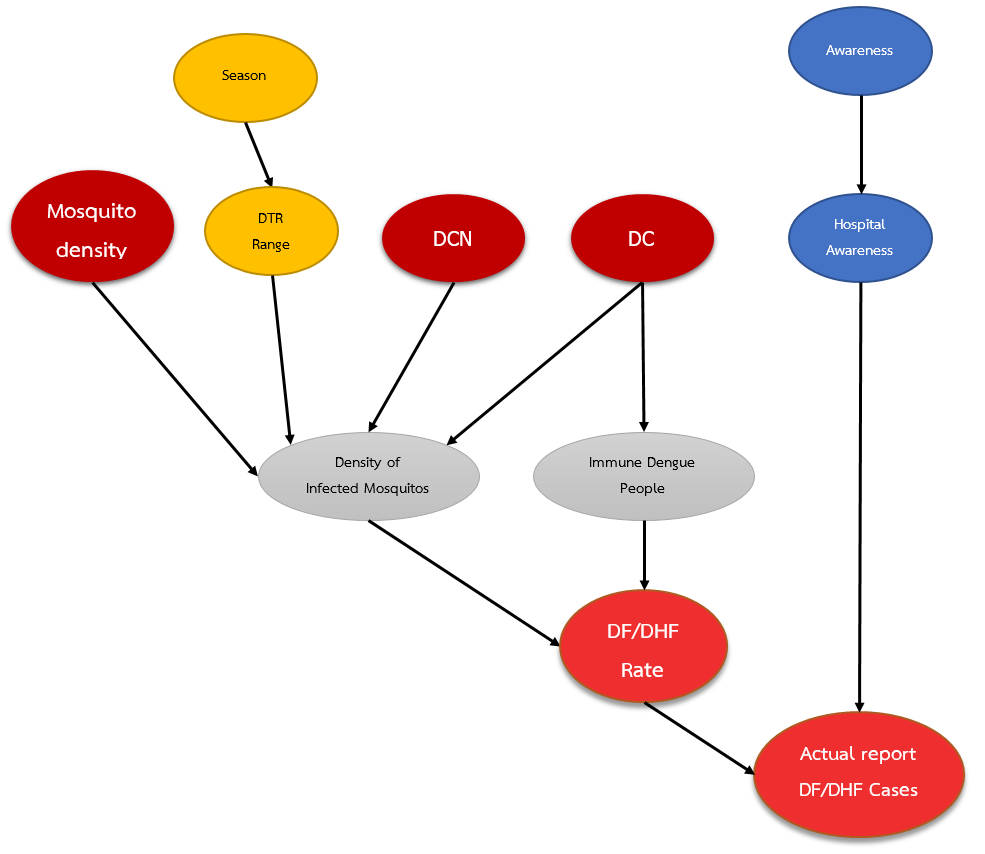
\includegraphics[width=150mm]{./figures/bn_df_rate}
		\caption{Directed acyclic graph of dengue incident rat Bayesian network model}
		\label{figure-bn-df-rate}
	\end{center}
\end{figure}

%\begin{table}[htbp]
%	\label{table-bn-dr-dag}
%	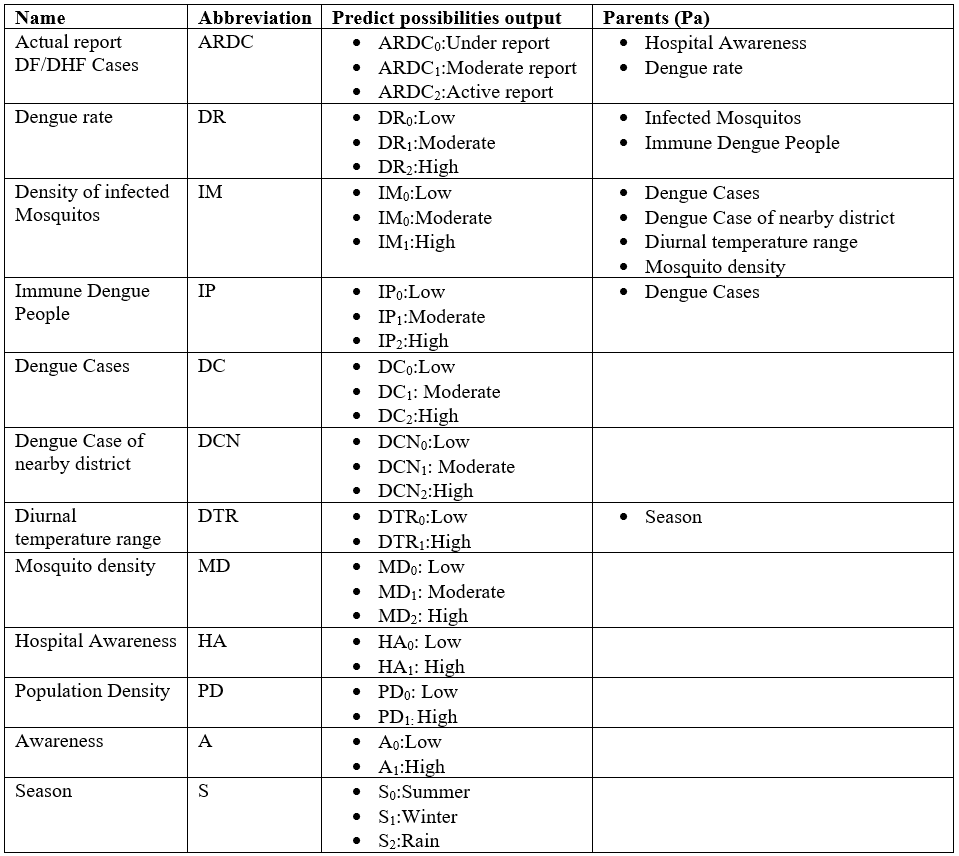
\includegraphics[width=150mm]{./figures/bn_dr_dag}
%	\caption{Value of each variables in dengue incident rate Bayesian network model}
%\end{table}


%\begin{table}[htbp]
%	\label{table-bn-dr-cpd}
%	\begin{center}
%		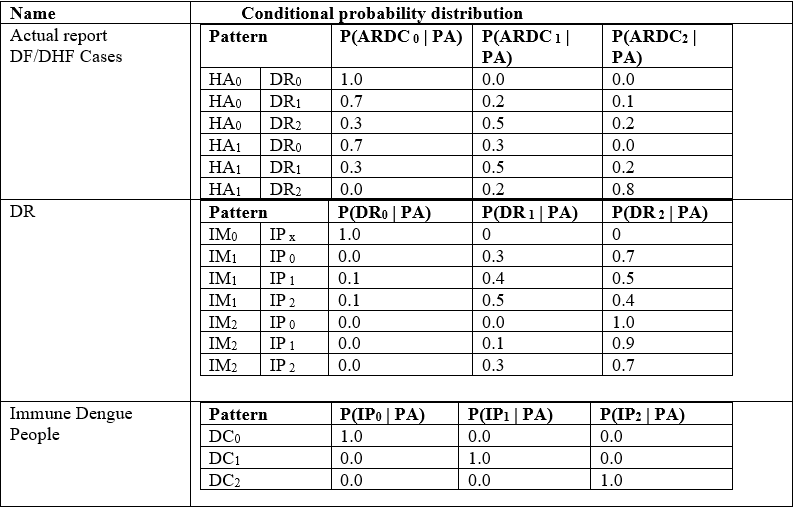
\includegraphics[width=120mm]{./figures/bn_dr_cpd_1}
%		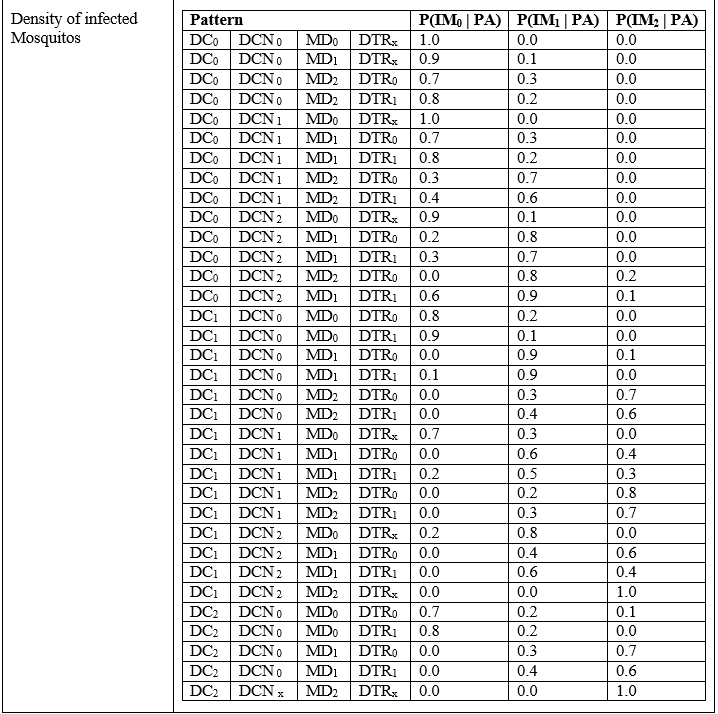
\includegraphics[width=121mm]{./figures/bn_dr_cpd_2}
%	\end{center}
%	\caption{Conditional probability distribution of each variables in dengue incident rate Bayesian network model}
%	
%\end{table}

Lastly, I combine both models into one model as shown in Digure \ref{figure-bn_md_dr}. 

\begin{figure}[htbp]
	\begin{center}
		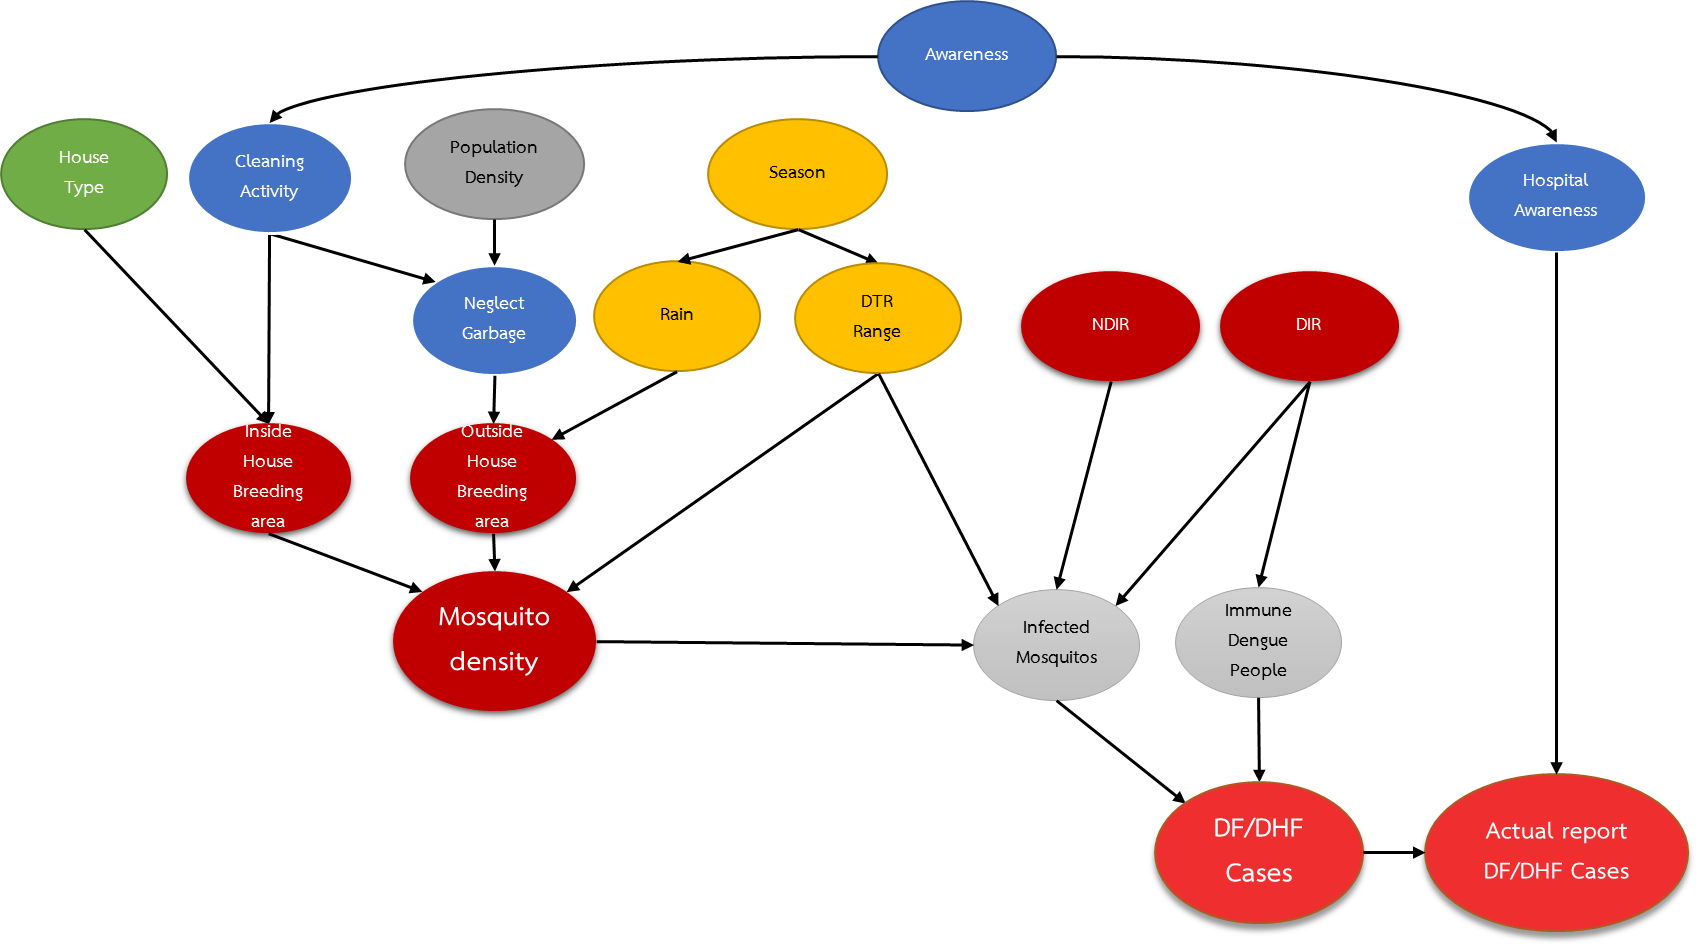
\includegraphics[width=150mm]{./figures/bn_md_dr}
		\caption{Combined directed acyclic graph of dengue incident rate and mosquito density Bayesian network model}
		\label{figure-bn_md_dr}
	\end{center}
\end{figure}


\section*{References}

\bibliography{mybibfile}


\end{document}